\newcommand{\dsize}{width=\textwidth, height=6cm, keepaspectratio}

\chapter{Modellierung}
\label{chap:Modellierung}
In diesem Kapitel wird die Modellierung des Frequenzumfomers beschrieben. Dazu werden folgende Anforderungen an das Modell gestellt:
\begin{itemize}
    \item Universales Modell des Frequenzumformers, zur \begin{itemize}
        \item Untersuchung der Ausgangsspannung bei Lastsprüngen
        \item Untersuchung des Einflusses der Maschinenparameter
        \item Untersuchung des Einflusses der Reglerparameter
    \end{itemize}
    \item Daraus folgt: \begin{itemize}
        \item Korrekte Wiedergabe der übertragenen Leistung
        \item Dynamische Eigenschaften werden so gut wie möglich wiedergegeben
    \end{itemize}
    \item Vernachlässigung folgender Punkte ist möglich: \begin{itemize}
        \item Anfahrverhalten
        \item Temperatureinflüsse
        \item Wirkungsgrad
    \end{itemize}
    \item Erweiterung und Anpassung des Modells / der Teilmodelle ist möglich
\end{itemize}

\section{Übersicht - Energie- und Informationsfluss}\label{sec:uxfcbersicht---energie--und-informationsfluss}

Bevor das Simulationsmodell in \textsc{Modelica} implementiert werden soll, ist es hilfreich, zunächst einen Überblick über das Gesamtsystem „rotierender Frequenzumformer“ zu erlangen und die Wirkungseinflüsse der einzelnen Größen zu studieren.

\subsection{Gesamtsystem}\label{sec:gesamtsystem}

Bei der betrachteten Anlage handelt es sich im Wesentlichen um einen Motor-Generator-Verbund aus einem Asynchronmotor und einem mit einer Synchron-Erregermaschine erregten Synchrongenerator. Das System besteht also aus drei mechanisch gekoppelten elektrischen Maschinen. Der Zusammenhang zwischen den elektrischen Größen am Stator und am Rotor der elektrischen Maschinen sowie die Kopplung mit der rotatorischen Bewegung wird über das Induktionsgesetz durch die Spannung und den Fluss des magnetischen Feldes charakterisiert.

\begin{figure}
    \centering
    \input{Tikz-Bilder/control.tikzstyles}
\begin{tikzpicture}[
    node distance=1cm
    ]
    % Asynchronmaschine
    \node (Netz_in) [bgelement] {Netz-Eingang};
    \node (ASM_Stator) [bgelement, below=of Netz_in] {Stator};
    %\node (ASM_Stator_R) [bgelement, above left=of ASM_Stator] {R};
    %\node (ASM_Stator_L) [bgelement, below left=of ASM_Stator] {L};
    \node (ASM_Luftspalt) [bgelement, below=of ASM_Stator] {Luftspalt};
    \node (ASM_Rotor) [bgelement, below=3cm of ASM_Luftspalt] {Rotor};
    %\node (ASM_Rotor_R) [bgelement, above left=of ASM_Rotor] {R};
    %\node (ASM_Rotor_L) [bgelement, below left=of ASM_Rotor] {L};
    \draw[bonds]
    (Netz_in) edge[flow=$i_{\mathrm{ein}}$, effort=$u_{\mathrm{ein}}$] (ASM_Stator)
    (ASM_Stator) %edge (ASM_Stator_R)
                 %edge (ASM_Stator_L)
                 edge[flow=$\Phi_{\mathrm{s}}$, effort=$V_{\mathrm{m,s}}$] (ASM_Luftspalt)
    (ASM_Luftspalt) edge[flow=$\Phi_{\mathrm{r}}$, effort=$V_{\mathrm{m,r}}$] (ASM_Rotor);
    %(ASM_Rotor) edge (ASM_Rotor_R)
    %            edge (ASM_Rotor_L);
    
    % Mechanik
    \node (Welle) [bgelement, right=1.1cm of ASM_Rotor] {Welle};
    % \node (Reibung) [bgelement, below =of Welle] {Reibung};
    
    \node (Gleichrichter) [bgelement, right=1cm of Welle] {Gleichrichter};
    \draw[bonds] 
        (ASM_Rotor) edge[effort=$M_{\mathrm{Motor}}$, flow=$\omega$] (Welle);
        % (Welle) edge[effort=$M_{\mathrm{Verl.}}$, flow=$\omega$] (Reibung);
    
     % Synchro-Generator
    \node (SG_Luftspalt) [bgelement] at (Gleichrichter|-ASM_Luftspalt.base) {Luftspalt};
    \node (SG_Rotor_Y) [between= Gleichrichter and SG_Luftspalt] {};
    \node (SG_Rotor) [bgelement] at (Gleichrichter|-SG_Rotor_Y) {Rotor};
    %\node (SG_Rotor_R) [bgelement, above right=of SG_Rotor] {R};
    %\node (SG_Rotor_L) [bgelement, below right=of SG_Rotor] {L};
    \node (SG_Stator) [bgelement] at (SG_Luftspalt|-ASM_Stator.base) {Stator};
    %\node (SG_Stator_R) [bgelement, above right=of SG_Stator] {R};
    %\node (SG_Stator_L) [bgelement, above left=of SG_Stator] {L};
    \draw[bonds]
    (Welle) edge[effort=$M_{\mathrm{Gen.}}$, flow=$\omega$] (SG_Rotor)
    (Gleichrichter) edge[effort=$u_{\mathrm{DC}}$, flow=$i_{\mathrm{DC}}$] (SG_Rotor)
    (SG_Rotor) edge[flow=$\Phi_{\mathrm{r}}$, effort=$V_{\mathrm{m,r}}$] (SG_Luftspalt)
               %edge (SG_Rotor_R)
               %edge (SG_Rotor_L)
    (SG_Luftspalt) edge[flow=$\Phi_{\mathrm{s}}$, effort=$V_{\mathrm{m,s}}$] (SG_Stator);
    %(SG_Stator) edge (SG_Stator_R)
    %            edge (SG_Stator_L);
    
    % Erregermaschine
    \node (EM_Rotor) [bgelement, below=of Gleichrichter] {Rotor};
    %\node (EM_Rotor_R) [bgelement, below left=of EM_Rotor] {R};
    %\node (EM_Rotor_L) [bgelement, below right=of EM_Rotor] {L};
    \node (EM_Luftspalt) [bgelement, right=of EM_Rotor] {Luftspalt};
    \node (EM_Stator) [bgelement, right=of EM_Luftspalt] {Stator};
    %\node (EM_Stator_R) [bgelement, below left=of EM_Stator] {R};
    %\node (EM_Stator_L) [bgelement, below right=of EM_Stator] {L};
    
    \draw[bonds]
    (Welle) edge[effort=$M_{\mathrm{Err.}}$, flow=$\omega$] (EM_Rotor)
    (EM_Rotor) edge[effort=$u_{\mathrm{AC}}$, flow=$i_{\mathrm{AC}}$] (Gleichrichter)
               %edge (EM_Rotor_L)
               %edge (EM_Rotor_R)
    (EM_Luftspalt) edge[flow=$\Phi_{\mathrm{r}}$, effort=$V_{\mathrm{m,r}}$] (EM_Rotor)
    (EM_Stator) edge[flow=$\Phi_{\mathrm{s}}$, effort=$V_{\mathrm{m,s}}$] (EM_Luftspalt);
                %edge (EM_Stator_R)
                %edge (EM_Stator_L);
    
    % Last
    \node (Last) [bgelement] at (EM_Stator|-SG_Stator) {Last};
    \draw[bonds] (SG_Stator) edge[flow=$i_{\mathrm{aus}}$, effort=$u_{\mathrm{aus}}$] (Last);
    
    % Regler
    \node (Summe) [sum, below=of Last] {};
    \node (Sollspannung) [input, right=of Summe, label=$U_{\mathrm{aus,soll}}$] {};
    \node (Regler) [block, label={right:}] at ($(Summe)!1/3!(EM_Stator)$) {PID};
    \node (PWM) [pulse, label={right:PWM}] at ($(Summe)!2/3!(EM_Stator)$) {};
    \draw[signal] (Last) -- node[left] (U_Regler_in) {$U_{\mathrm{aus,ist}}$} (Summe);
    \draw[signal] (Sollspannung) -- node[near end,below]{\small $-$} (Summe);
    \draw[signal] (Summe) -- (Regler);
    \draw[signal] (Regler) -- (PWM);
    \draw[bonds] (PWM) ++(0,-.6) edge[effort=$u_{\mathrm{err}}$, flow=$i_{\mathrm{err}}$] (EM_Stator);
    
    %Beschriftung
    \node [below=.3cm of EM_Luftspalt] {Erregermaschine};
    \node [above=.3cm of SG_Stator] {Synchrongenerator};
    \node [below=.3cm of ASM_Rotor] {Asynchronmaschine};
    \node [right=.3cm of Regler, align=center] {Regler-\\ board};
    \begin{pgfonlayer}{background}
    \filldraw [line width=4mm,join=round,black!5]
      (Netz_in.west|-Netz_in.north)  rectangle (Netz_in.east|-ASM_Rotor.south)
      (SG_Luftspalt.west|-SG_Stator.north) rectangle (SG_Luftspalt.east|-SG_Rotor.south)
      ($(EM_Rotor.west|-EM_Rotor.north) + (0,.1)$) rectangle ($(EM_Stator.east|-EM_Stator.south) + (0,-.1)$);
      %($(U_Regler_in.west) + (0,.2)$) rectangle ($(Sollspannung.east|-PWM.east) + (.4,-.4)$);
  \end{pgfonlayer}
\end{tikzpicture}
    \caption{Energie- und Informationsfluss des rotierenden Frequenzumformers. Die Angabe der Größen erfolgt mit Bezug auf Stator- ($s$) bzw. Rotorseite ($r$).}
    \label{fig:Wirkungsgraph}
\end{figure}

In Anlehnung an die Bondgraphen-Methode zeigt der „Wort-Bondgraph“ (oder „Wortgraph“, vgl. \cite[S.~10]{roddeckBondgraphenModellbildungUnd2019}) in \cref{fig:Wirkungsgraph} den Energie- und Informationsfluss im Frequenzumformer. Die Halbpfeile (\bond) repräsentieren den Energiefluss (die übertragene Leistung) der zusammenhängenden \emph{Fluss-} (\emph{Flow}) und \emph{Potential}größen (\emph{Effort}). Nach Konvention werden die Potentialgrößen oberhalb und die Flussgrößen unterhalb der Halbpfeils aufgetragen. 

Im Gegensatz zu den formalen Bondgraphen können die Knoten des Wortgraphen mehrere Größen und Verbindungen, die zum Aufstellen des Zustandsraummodells nötig wären, unter einem Oberbegriff zusammenfassen und vereinfachen (\emph{Objektorientierung}). Ist eine detaillierte Darstellung gesucht, können diese einzelnen Oberbegriffe jeweils durch ihre korrespondierenden Bondgraph-Darstellungen ersetzt werden. Bondgraphen für die einzelnen elektrischen Maschinen können beispielsweise \cite[S.~269~ff.]{borutzkyBondGraphModelling2011} entnommen werden.

Ursache für den in \cref{fig:Wirkungsgraph} dargestellten Energiefluss ist die Vorgabe der Spannung am Netz-Eingang. Sie bewirkt einen Stromfluss im Stator, der einerseits zur Wandlung elektrischer Energie in magnetische Energie führt, die über den Luftspalt auf den Rotor übertragen wird und andererseits mit der Abgabe von elektrischer und magnetischer Verlustenergie (ohm'sche Verluste Streufluss) verbunden ist. Der Luftspaltwirkt wie ein Transformator, der das Verhältnis der magnetischen Spannung zum Fluss bei der Übertragung auf den Rotor  wandelt. Im Rotor wird eine Spannung induziert, die einen Stromfluss zur Folge hat. Über die Lorentzkraft folgt die Wandlung in kinetische (rotatorische) Energie.

Während die Winkelgeschwindigkeit der Welle für angrenzenden Baugruppen gleich ist, teilt sich das Motormoment auf. Ein Teil der Energie wird über die Massenträgheit in der Welle gespeichert und ein Teil verlässt das System durch Reibungseffekte (Lagerreibung, Luftwiderstand, \ldots). Der größte Teil wird jedoch an den Synchrongenerator und die Erregermaschine übertragen.

Die Hauptaufgabe der Erregermaschine ist es, die Spannung am Ausgang des Reglersystems berührunglos auf den Rotor des Synchrogenerators zu übertragen. Dies geschieht durch Wandlung der elektrischen Energie und Übertragung über den Luftspalt der Maschine. Gekoppelt sind Generator und Erregermaschine über den mitrotierenden Gleichrichter. Der Synchrongenerator wandelt die eingebrachte mechanische Energie und die Erregung über den Luftspalt in elektrische Energie.

Zusätzlich zu dem Energiefluss ist in \cref{fig:Wirkungsgraph} auch der Informationsfluss angedeutet: Am Ausgang des Umformers wird der Spannungsabfall über der Last gemessen und die Differenz zum Sollwert in den Regler zurückgeführt. Der PID-Spannungsregler ist hier zusammengefasst dargestellt. Ein ausführliches Blockschaltbild des Reglers zeigt \cref{fig:Blockschaltbild_Regler}. Aus der vom Regler berechneten Stellgröße wird über Puls-Weiten-Modulation eines Steuertrafos die Statorspannung der Erregermaschine erzeugt.

\subsection{PID-Spannungsregler}\label{sec:pid-spannungsregler}

Als Spannungsregler wird in dem Frequenzumformer ein PID-Regler mit \emph{variabler Verstärkung} eingesetzt. Die variable Verstärkung dient zum Erreichen eines besseren Einschwingverhaltens bei großen Regelabweichungen (vgl. \cite{DigitalerSpannungsreglerSoftwaredokumentation}). \cref{fig:Blockschaltbild_Regler} zeigt das Blockschaltbild des Reglers. Der PID-Regler ist in Parallelstruktur ausgeführt; an den Ausgängen der Regelglieder und am Gesamtausgang werden die Stellgrößen begrenzt. 

\begin{figure}
    \centering
    \input{Tikz-Bilder/control.tikzstyles}
\begin{tikzpicture}[node distance=1.5cm]
		% I-Regulator
		\node [integral, label={below:I-Regler}] (I-Reg) at (0,0) {};
		\node [limiter] (I-Lim) [right of=I-Reg] {};
		\node [sum] (sum) [right of=I-Lim] {};
		\node [limiter] (All-Lim) [right of=sum] {};
		\node [pulse, label={[align=center] below:Pulsweiten-\\Modulator}] (PulseModulator) [right of=All-Lim] {};
		% D-Regulator
		\node [differential, label={below:D-Regler}] (D-Reg) [below of=I-Reg] {};
		\node [limiter] (D-Lim) [right of=D-Reg] {};
		% P-Regulator
		\node [proportional, label={below:P-Regler}] (P-Reg) [above of=I-Reg] {};
		\node [limiter] (P-Lim) [right of=P-Reg] {};
		% PP-Regulator
		\node [proportional, label={above:Gain-Regler}] (PP-Reg) [above of=P-Reg] {};
		\node [limiter] (PP-Lim) [right of=PP-Reg] {};
        \node (PP_h) at ($ (sum|-PP-Lim) + (0,-.6) $) {};
        % Input and Knots
		\node [splitter] (knot1) [left of=I-Reg] {};
		\node [splitter] (knot2) [left of=P-Reg] {};
		\node [input] (input) [left of=knot1] {};
        \node (output) [node distance=1.5cm, right of=PulseModulator]{};
        
        %% Edges
        \draw [signal] (input) -- (knot1) -- (I-Reg);
        % I-Regulator
        \draw [signal] (I-Reg) -- (I-Lim);
        \draw [signal] (I-Lim) -- (sum) node [xshift=-0.6cm, above] {\footnotesize$+$};
        % D-Regulator
		\draw [signal] (knot1) |- (D-Reg);
		\draw [signal] (D-Reg) -- (D-Lim);
		\draw [signal] (D-Lim) -| (sum) node [yshift=-0.6cm, left] {\footnotesize$+$};
		% P-Regulator
		\draw [signal] (knot1) |- (P-Reg);
		\draw [signal] (P-Reg) -- (P-Lim);
		\draw [signal] (P-Lim) -| (sum) node [yshift=0.6cm, right] {\footnotesize$+$};
		% PP-Regulator
		\draw [signal] (knot1) |- (PP-Reg);
		\draw [signal] (PP-Reg) -- (PP-Lim);
		\draw [signal] (PP-Lim) -| (PP_h.center) -| (P-Reg);
		% Output
		\draw [signal] (sum) -- (All-Lim);
		\draw [signal] (All-Lim) -- (PulseModulator);
		\draw [signal] (PulseModulator) -- (output);
\end{tikzpicture}
    \caption{Blockschaltbild des Reglers, eigene Darstellung nach \cite{piller_power_systems_gen_bsb11_1999}}
    \label{fig:Blockschaltbild_Regler}
\end{figure}

Implementiert ist der PID-Regler als digitaler Regler auf einem Mikrocontroller. Dabei sind einige Punkte zu beachten:
\begin{itemize}
    \item {Die Algorithmen für die Regelglieder arbeiten zeitdiskret. Zur Ableitung der Algorithmen muss die Abtastung mit einem ZOH-Glied beim Anwenden der $\mathcal{Z}$-Transformation berücksichtigt werden, siehe \cref{par:ZeitdiskreterRegler}.}
    \item {Die Abtastung der Ausgangsspannung erfolgt nach \cite{DigitalerSpannungsreglerSoftwaredokumentation} bei dem hier betrachteten Spannungsregler mit 32 Messwerten in 5 Taktzyklen, wobei sich die Taktfrequenz nach der Frequenz der Ausgangsspannung richtet. Die Abtastrate für die Spannungsmessung beträgt also
    \begin{align}
        T_{\mathrm{mess}}^*&= \frac{5}{32}\cdot T_{\mathrm{Spannung}} = 0,000390625\,\mathrm s. \\
        \text{mit} \quad
        T_{\mathrm{Spannung}}&= \frac{1}{400\,\mathrm{Hz}}=0,0025\,\mathrm s
    \end{align}
    Weiterhin gibt \cite{DigitalerSpannungsreglerSoftwaredokumentation} an, dass bei einer Spannungsfrequenz von \(f=400\,\mathrm{Hz}\) der Regelalgorithmus nur alle zwei Messzyklen neu berechnet wird. Die Periodendauer des zeitdiskreten Reglers beträgt also
    \begin{align}
        T_{mess}&=2\cdot T_{mess}^*= 0,00078125\,\mathrm s.
    \end{align} }
    \item {Die Digitalisierung der Spannungsmessung bedeutet eine Quantisierung der Werte. Die gemessenen Werte werden Reglerintern auf \(2^{16}\) ganzzahlige vorzeichenbehaftete Werte (\emph{``16 bit signend integer''}) abgebildet, also auf das Intervall \([-32768,32767]\). Um den Zusammenhang zwischen der realen Spannung und der internen Darstellung herzustellen, müssen Umrechnungsfaktoren angegeben werden.}
\end{itemize}


\section{Umsetzung}\label{sec:umsetzung}

Die im Folgenden beschriebene Modellierung des Frequenzumformers erfolgt auf Basis der \modclass{Modelica\ Standard\ Library\ v3.2.3} (MSL, siehe \cite[]{modelicaassociationModelicaStandardLibrary2020}). So weit nicht anders angegeben sind alle im Folgenden behandelten Bibliotheken und Klassen der MSL entnommen. Für das entwickelte Modell und benötigte Hilfsklassen wird eine eigenständige Bibliothek \modclass{Frequenzumformer} angelegt. Alle Klassen, die dieser Bibliothek angehören, werden mit \modclass{Frequenzumformer.Klasse} bezeichnet. Die vollständige Bezeichnung der abgeleiteten Klassen zeigt die Hierarchie der jeweiligen Bibliothek. Beginnend bei dem Bibliotheksnamen wird jedes untergeordnete Objekt mit einem Punkt abgetrennt angefügt, z.B. \modclass{Modelica.Bibliothek.Unterobjekt}.

Für den Asynchronmotor und den Synchrongenerator werden die Modelle \modclass{AIM\_­Squir­rel­Cage} und \modclass{SM\_ElectricalExcited} aus der Bibliothek \modclass{Mag\-netic.\-Funda\-men\-tal\-Wave} der MSL verwendet. Die Herleitung dieser Modelle ist umfangreich in \cite[]{kralModelicaObjektorientierteModellbildung2019} beschrieben und soll hier nur kurz zusammengefasst werden. Verwendet werden die jeweiligen transienten elektrischen Komponenten und Maschinen, da nur mit diesen Einschwingvorgänge beobachtet werden können. Die quasi-stationären Modelle (Klassen in den Paketen \modclass{Electrical.QuasiStationary} und \modclass{Magnetic.QuasiStatic}) verwenden zur Berechnung der elektrischen und magnetischen Größen komplexe Zeiger. Diese sind nicht geeignet zur Untersuchung von Einschwingvorgängen, da die Zeiger aus der Fourier-Transformation periodischer eingeschwungener Größen hergeleitet werden.

Nach \cite[S. 149]{kralModelicaObjektorientierteModellbildung2019} werden für die betrachteten Maschinen in der MSL folgende Voraussetzungen und Vereinfachungen getroffen:
\begin{itemize}
	\item Die Wicklungen sind vollständig symmetrisch ausgeführt.
	\item Oberwellen der magnetischen Größen im Luftspalt werden vernachlässigt.
	\item Sättigungseffekte werden vernachlässigt.
\end{itemize}

\subsection{Asynchronmotor mit Kurzschlussläufer}\label{sec:asynchronmotor-mit-kurzschlussluxe4ufer}
Da die betrachteten Drehfeldmaschinen in vielen Bereichen gleich oder zumindest ähnlich aufgebaut sind, legt \cite{kralModelicaObjektorientierteModellbildung2019} den Asynchron- und Synchronmaschinen der MSL ein \emph{partielles \textsc{Modelica}-Modell} für Drehfeldmaschinen zugrunde (\modclass{FundamentalWave.­In­ter­fa­ces.­Par­tial­Ba­sic­In­duc­tion­Ma­chine}). Das unterstützt den objektorientierten Modellierungsansatz, sodass diese Grundstruktur nicht für jede elektrische Maschine neu aufgestellt werden muss. Ein solches partielles (Modifizierer \modclass{partial}) Modell muss nicht die gleiche Anzahl von Gleichungen und Unbekannten implementieren und kann daher nicht allein simuliert werden. Es bietet die Möglichkeit, Strukturen des Modells bei der Vererbung zu verändern (\modclass{replace}).

\subsubsection{Partielles Modell der Drehfeldmaschine}\label{sec:partielles-modell-der-drehfeldmaschine}
Das partielle Modell der Drehfeldmaschine (siehe \cref{fig:partiellDrehfeldmaschinen}) modelliert die Energieübertragung vom elektrischen Netzanschluss des Stators über den Luftspalt auf den Rotor, wie sie schon in \cref{fig:Wirkungsgraph} betrachtet wurde. Die Ausgestaltung des Rotormodells und der mögliche Anschluss elektrischer Klemmen an den Rotor (z.B. über Schleifringe) ist dann Teil der Spezialisierung des Modells für die einzelnen elektrischen Maschinen. Neben der Stator-Rotor-Kopplung bietet das partielle Modell auch einen Sammelpunkt für Wärmeenergie aller Teilkomponenten, eine mechanische Trägheitskomponente für die Trägheit des Rotors der Maschine verbunden mit einem Lagerreibungsmodell und einem optionalen mechanischen Anschluss zur Abstützung des Stators.

\begin{figure}
\centering
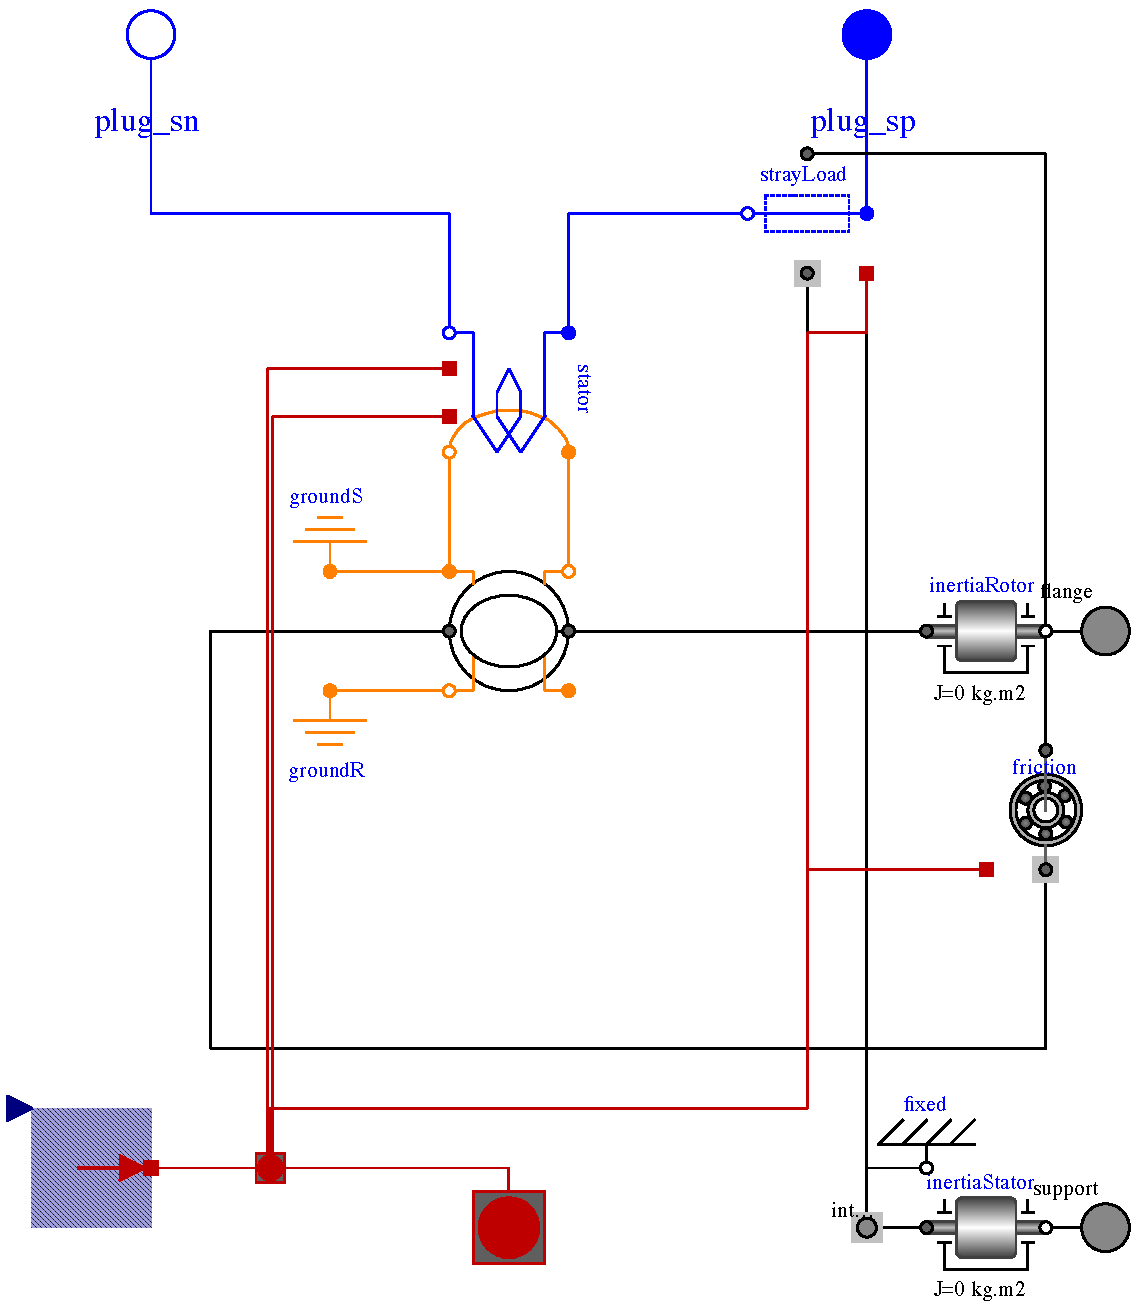
\includegraphics[height=6cm]{Bilder/PartialBasicInductionMachine.pdf}
\caption{Partielles Modell der Drehfeldmaschine \modclass{Fun­da­men­tal­Wave.­In­ter­fa­ces.­PartialBasicInductionMachine} der MSL v3.2.3}
\label{fig:partiellDrehfeldmaschinen}
\end{figure}

Die Energiewandlung im Stator geschieht über das Windungsmodell \modclass{Fun­da­men­tal­Wave.­Ba­sic­Ma­chines.­Com­po­nents.­Sym­me­tric­Mu­lti­Phase­Win­ding}, welches neben der elektro\-mag\-ne\-ti\-schen Kopplung auch ohmsche Verluste sowie Streu- und Wirbelstromverluste des Magnetfelds berücksichtigt. Außerdem berücksichtigt das Modell  bei ungeradzahligen mehrphasigen Systemen noch die Nullinduktivität. Das wird jedoch nur benötigt, wenn die Windung unsymmetrisch belastet wird (\cite[S. 193]{kralModelicaObjektorientierteModellbildung2019}), was in der hier betrachteten Anwendung nicht auftritt.

% \begin{figure}
% \centering
% 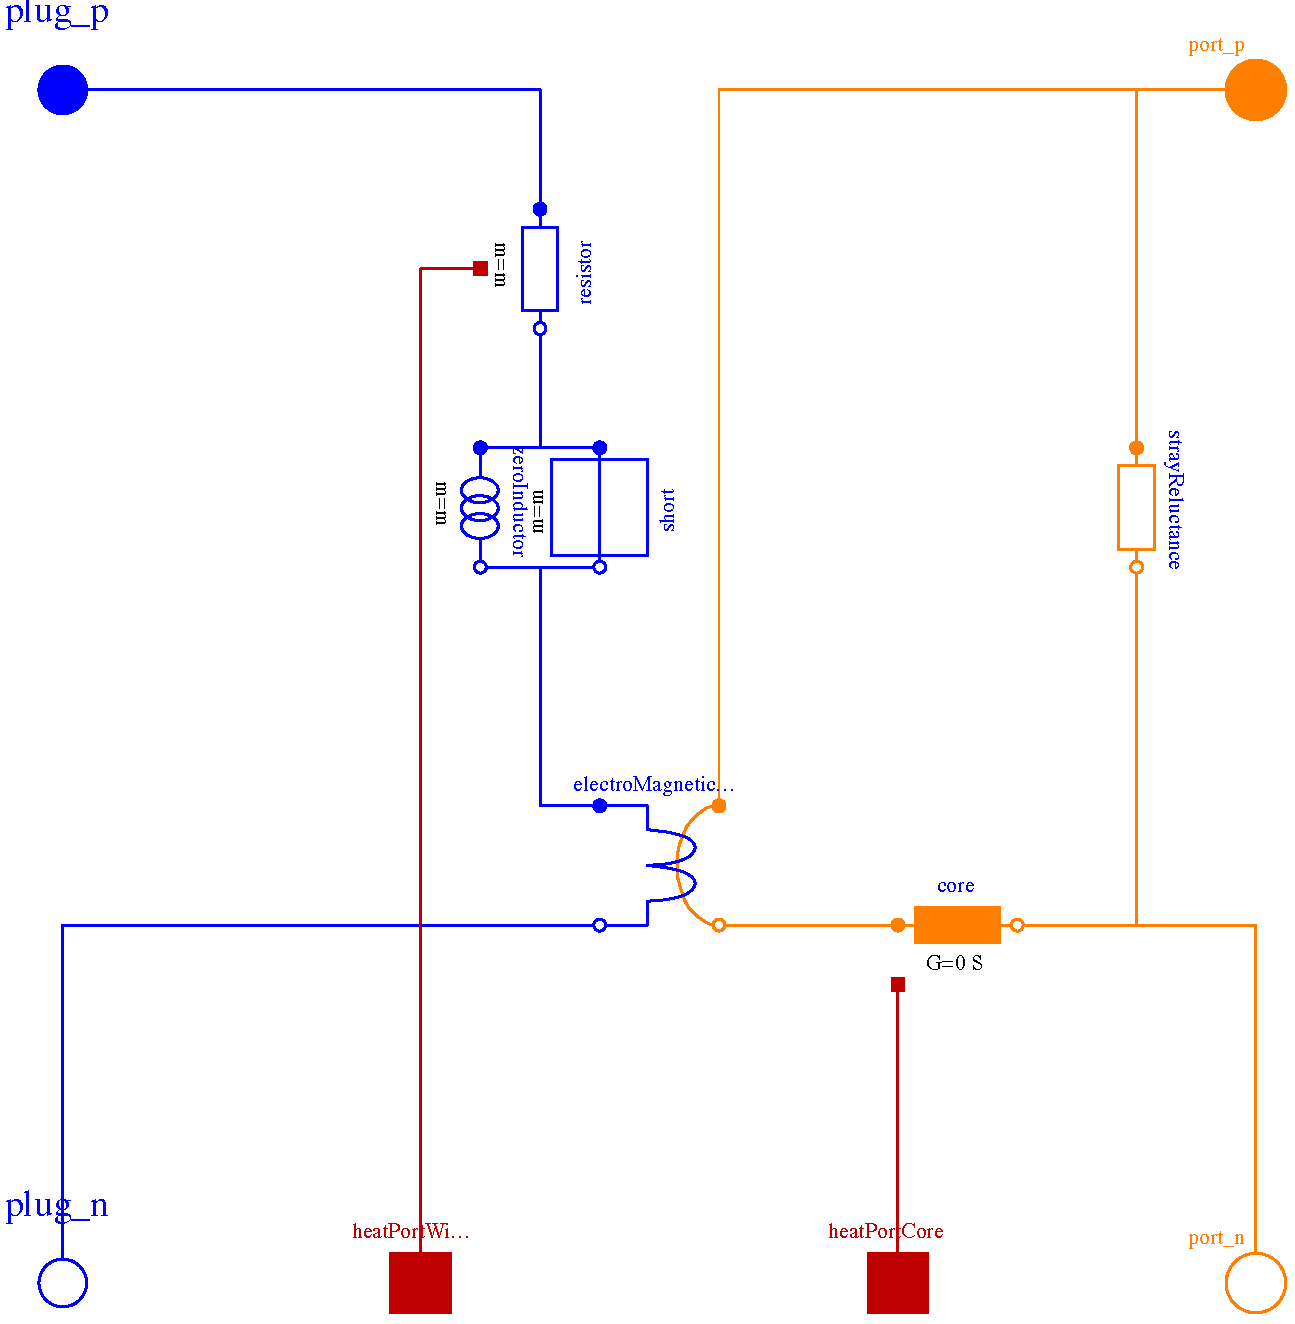
\includegraphics[height=6cm]{Bilder/SymmetricMultiPhaseWinding.pdf}
% \caption{Windungsmodell \modclass{FundamentalWave.Basic­Ma­chines.­Com­po­nents.­Sym­me­tric­Mu­lti­Phase­Win­ding}
% der MSL v3.2.3}
% \label{fig:MultiPhasenWindung}
% \end{figure}

Über das Luftspaltmodell (\modclass{FundamentalWave.BasicMachines.­Com­po­nents.­Ro­tor­Sa­li­en­cy­Air­Gap}) wird der Abfall der magnetischen Spannung über dem magnetischen Widerstand des Luftspalts sowie das auf den Rotor wirkende Drehmoment modelliert. Um die magnetischen Größen des Stators und des Rotors in Beziehung zueinander zu setzen, ist eine Koordiantentransformation der Statorgrößen in das körperfeste Bezugssystem des Rotors implementiert (\emph{d,q-System}).

\hypertarget{sec:modell-ASM}{%
\subsubsection{Modell}\label{sec:modell-ASM}}

Das vollständige Modell der Asynchronmaschine mit Kurzschlussläufer (\modclass{Fun­da­men­tal­Wave.­Ba­sic­Ma­chines.­A­syn­chro­nous­In­duc­tion­Ma­chines.­AIM­\_­Squir­rel­Cage}) zeigt \cref{fig:ASM_vollstaendig}. Es ergibt sich aus dem partiellen Modell durch Hinzufügen des kurzgeschlossenen Käfigmodells (\modclass{Fun­da­men­tal­Wave.Ba­sic­Ma­chines.­Com­po­nents.­Sym­me­tric­Mul­ti­Phase­Cage­Win­ding}).

Da die Anzahl \(N_{\mathrm{R}}\) der Rotorstäbe eines Käfigs häufig viel größer ist als die Anzahl (m) der Phasen des Systems, ist es numerisch einfacher für den Käfig eine (m)-phasige kurzgeschlossene Windung als Ersatzmodell zu verwenden, welche die gleiche effektive Windungszahl wie die Statorwicklung aufweist. (\cite[S. 194]{kralModelicaObjektorientierteModellbildung2019})

\begin{figure}
\centering
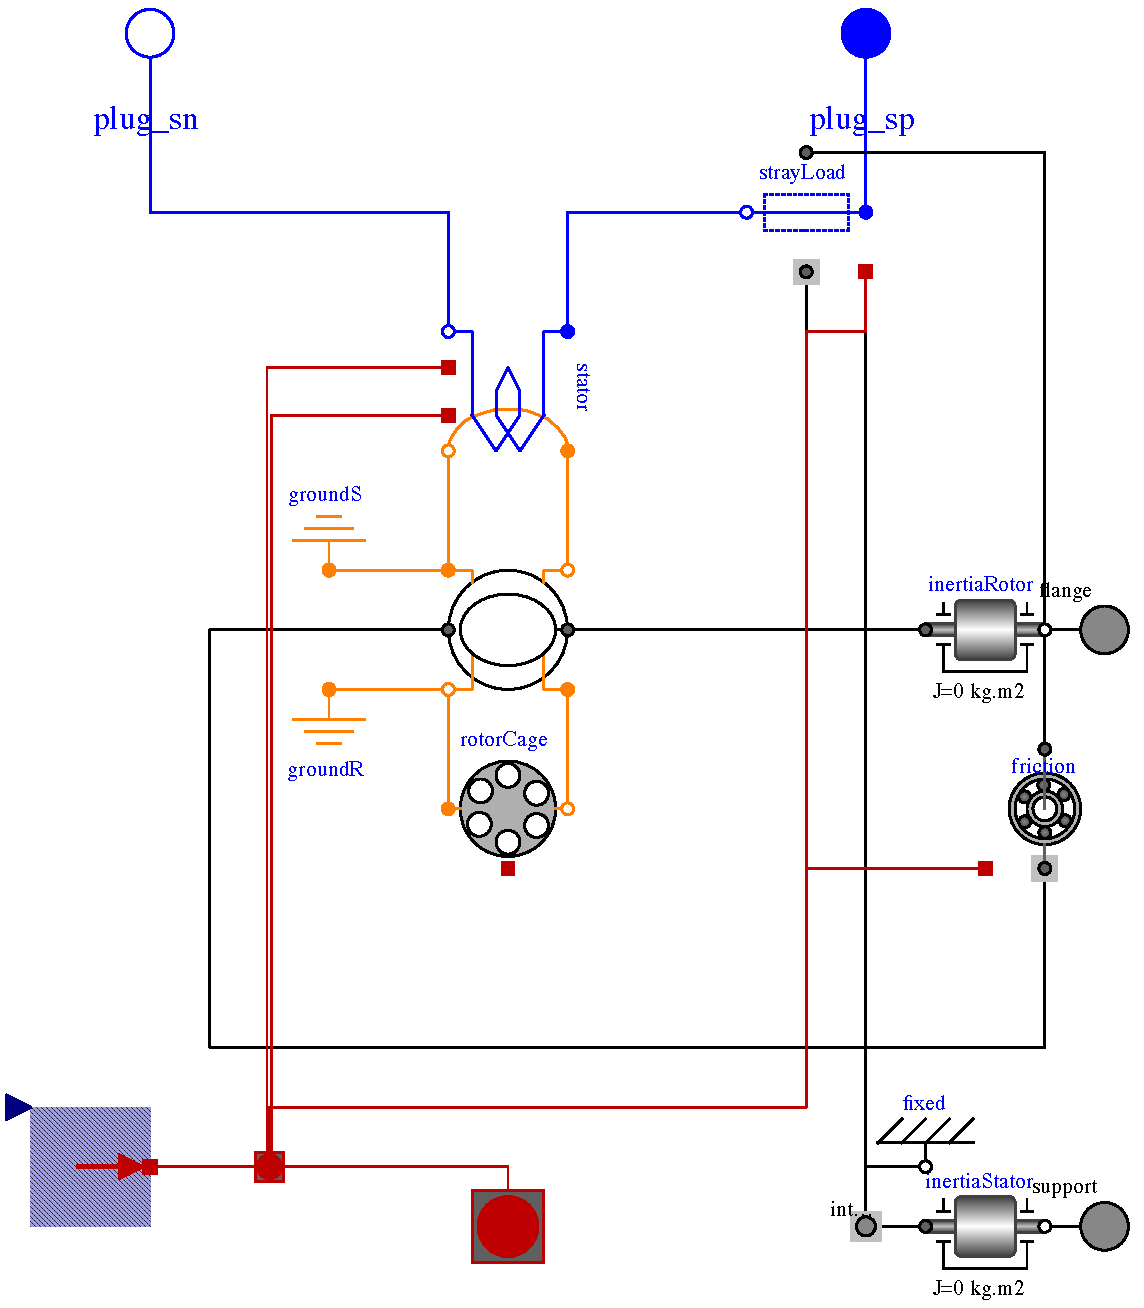
\includegraphics[height=8cm]{Bilder/AIM_SquirrelCage.pdf}
\caption{Vollständiges Modell der Asynchronmaschine mit Kurzschlussläufer (\modclass{Fun­da­men­tal­Wave.­Ba­sic­Ma­chines.­A­syn­chro­nous­In­duc­tion­Ma­chines.­AIM\_­Squir­rel­Cage}) der MSL v3.2.3}
\label{fig:ASM_vollstaendig}
\end{figure}

% \begin{figure}
% \centering
% 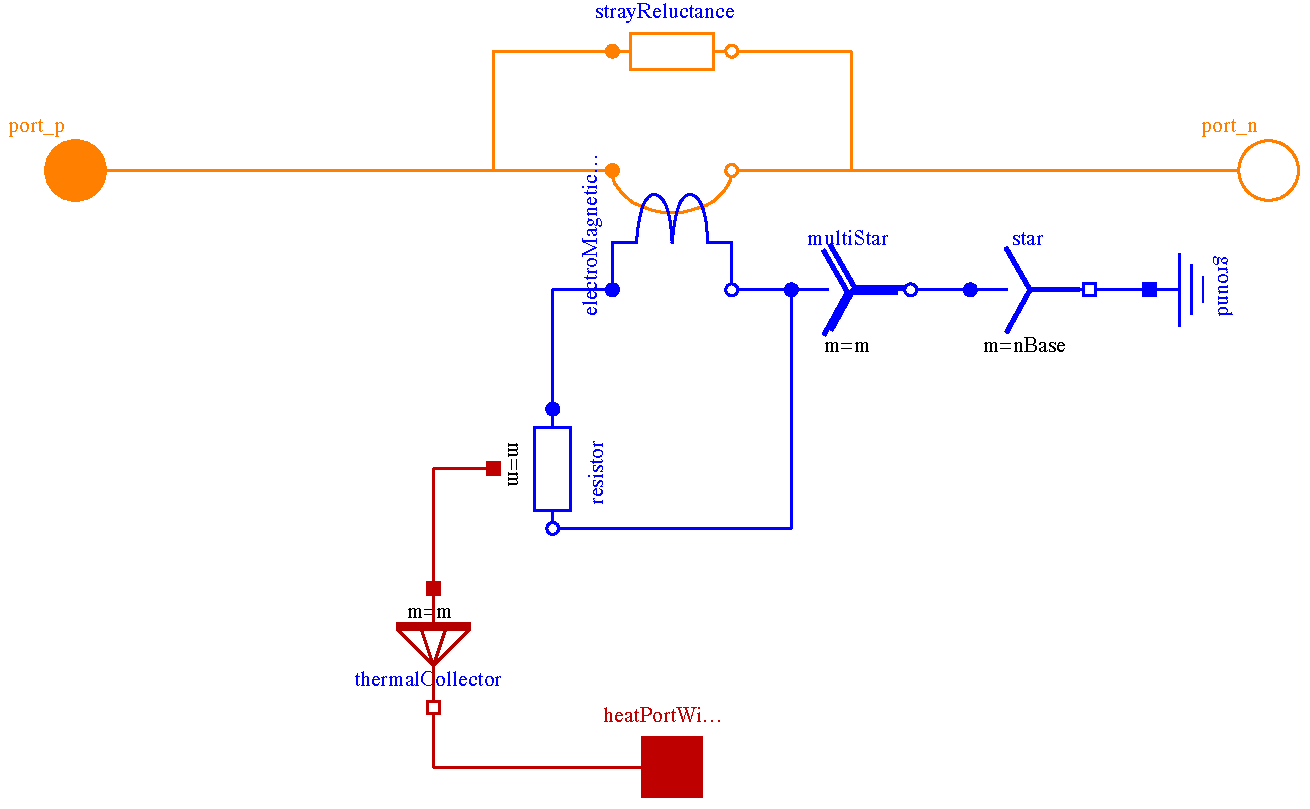
\includegraphics[]{Bilder/SymmetricMultiPhaseCageWinding.pdf}
% \caption{M-phasiges Käfig-Ersatzmodell (\modclass{Fun­da­men­tal­Wave.­Com­po­nents.­Sym­metric­Mul­ti­Phase­Cage­Win­ding}) der MSL v3.2.3}
% \label{fig:MPhasigerKaefig}
% \end{figure}

\subsubsection{Parametrierung}\label{sec:parametrierung-ASM}

Zur Parametrierung der Maschine müssen drei Arten von Größen angegeben werden: elektrische, mechanische und thermische Größen. Da bei Adaptieren des Fre­quenz­um­for­mer-Modells auf andere Maschinengrößen vorrangig die elektrischen und mechanischen Größen angepasst werden müssen, werden diese Werte in einem eigenen Record-Modell (\modclass{Frequenzumformer.Maschinenparameter.AIM\_­Squir­rel­Cage­Da­ta}, siehe \cref{lst:RecordASMData}) zusammengefasst. Das ermöglicht auch die Umrechnung der im Datenblatt der Maschine angegebenen Reaktanzen in die für die Simulation benötigten Induktivitäten.

Die thermischen Größen (Betriebspunkts- und Referenztemperaturen von Stator und Rotor, Temperaturabhängigkeit der Widerstände) werden auf \unit[20]{°C} Umgebungstemperatur eingestellt, wobei die Temperaturabhängigkeit der Widerstände vernachlässigt werden soll.

Wie schon oben erwähnt, verwendet das Modell der Asynchronmaschine nach außen hin zur Parametrierung der Wicklungen Stator- und Rotorinduktivitäten, sowie die effektive Statorwindungszahl. Die Induktivitäten sind die auch im T-Ersatzschaltbild der Maschine (vgl. \cref{fig:ESB_ASM}) angegeben Größen: Hauptfeldinduktivität (\(L_m\)), Stator-Streuinduktivität (\(L_{s\sigma}\)) und Rotor-Streuinduktivität (\(L_{r\sigma}\)). Im Datenblatt der Maschine sind die Reaktanzen \(X_0, X_1, X_2\) angegeben. Die zugehörigen Induktivitäten ergeben sich mit der Netzfrequenz \(f_{Netz}=\unit[50]{\mathrm{Hz}}\) nach
\begin{align}
    L_m &= \frac{X_0}{2\pi f_{Netz}} \\
    L_{s,\sigma} &= \frac{X_1}{2\pi f_{Netz}} \\
    L_{r,\sigma} &= \frac{X_2}{2\pi f_{Netz}}.
\end{align}
Für die effektive Windungszahl (\modclass{effectiveStatorTurns}) gibt \cite[S. 217]{kralModelicaObjektorientierteModellbildung2019}
\begin{equation}
    N_{\mathrm{eff. s}} = \hat{N}\cdot\xi_{\mathrm{c}}\cdot\xi_{\mathrm{z}}\label{eq:effStatorTurns},
\end{equation}
an, mit der \emph{Statorwindungszahl} \(\hat{N}\), dem \emph{Sehnungsfaktor} \(\xi _{\mathrm{c}}\) und dem \emph{Zonenfaktor} \(\xi _{\mathrm{z}}\). Ebenda angegeben sind die \cref{eq:xic,eq:xiz} für die beiden Faktoren \(\xi _{\mathrm{c}}\) und \(\xi_{\mathrm{z}}\) (\cite[S. 165, S. 217]{kralModelicaObjektorientierteModellbildung2019}).
\begin{align}
    \xi _{\mathrm{c}} &= \sin(\frac{\Delta\gamma _{\mathrm{c}}}{2}) \label{eq:xic}\\
    \xi _{\mathrm{z}} &= \frac{\sin(\frac{\pi}{6})}{q\sin(\frac{\pi}{6q})}\label{eq:xiz}
\end{align}
Die \emph{Spulenweite} \(\Delta\gamma _{\mathrm{c}}\) ist gemäß
\begin{equation}
    \Delta\gamma _{\mathrm{c}} = 2\pi\cdot\frac{y _{\mathrm{Q}}}{S'}
\end{equation}
das Verhältnis des \emph{Nutschritts} (\(y_Q\)) zur Anzahl der \emph{Nuten je Polpaar} (\(S'=\nicefrac{Q}{2p}\)) multipliziert mit \(2\pi\) (\cite[S. 168, S. 161]{kralModelicaObjektorientierteModellbildung2019}), vgl. \cite[S. 76, S. 119]{binderElektrischeMaschinenUnd2012}). Ebenso ist die \emph{Lochzahl} (\(q\)) zur Berechnung des Zonenfaktors das Verhältnis der Anzahl der Nuten zur Anzahl der Stränge und Pole (vgl. \cite[S. 151]{kralModelicaObjektorientierteModellbildung2019})
\begin{equation}
    q = \frac{Q}{2pm}\label{eq:Lochzahl}.
\end{equation}
Damit ist die Statorwindung der Asynchronmaschine vollständig parametriert. Die Wicklungsdaten und die daraus nach \crefrange{eq:effStatorTurns}{eq:Lochzahl} berechneten Werte listet \cref{tab:WicklungsdatenASM} auf. Alle weiteren Größen zur Beschreibung der Asynchronmaschine können direkt aus dem Datenblatt entnommen werden und sind ebenfalls in \cref{tab:ParameterASM,tab:WerteParameterrecordASM} angegeben. 

Dabei ist für das Trägheitsmoment \(J_{\mathrm{r}}=0\) eingetragen, da aus der Auslegung des Frequenzumformers nur ein kombiniertes Trägheitsmoment der Welle mit den Rotoren aller drei Maschinen und dem Lüfter bekannt ist. Da die Modellierung der Welle starr (d.h. ohne Berücksichtigung der Elastizität oder der inneren Dämpfung der Welle) geschieht, kann dieses kombinierte Trägheitsmoment im Trägheitsmoment des Lüftermodells zusammengefasst werden.

\subsection{Synchrongenerator mit Dämpferkäfig}\label{sec:synchrongenerator}

Auch das Modell des Synchrongenerators basiert wie das der Asynchronmaschine auf dem oben schon dargestellten partiellen Drehfeldmaschinenmodell. Es fügt dem partiellen Modell ein einphasiges elektro-magnetisches Kopplungsmodell und ein Bürstenmodell für die elektrische Erregung hinzu und bietet einen optionalen Dämpferkäfig, ähnlich zu dem Kurzschlussläufer der Asynchronmaschine.

\hypertarget{sec:Modell-SG}{%
\subsubsection{Modell}\label{sec:Modell-SG}}
\begin{figure}
    \centering
    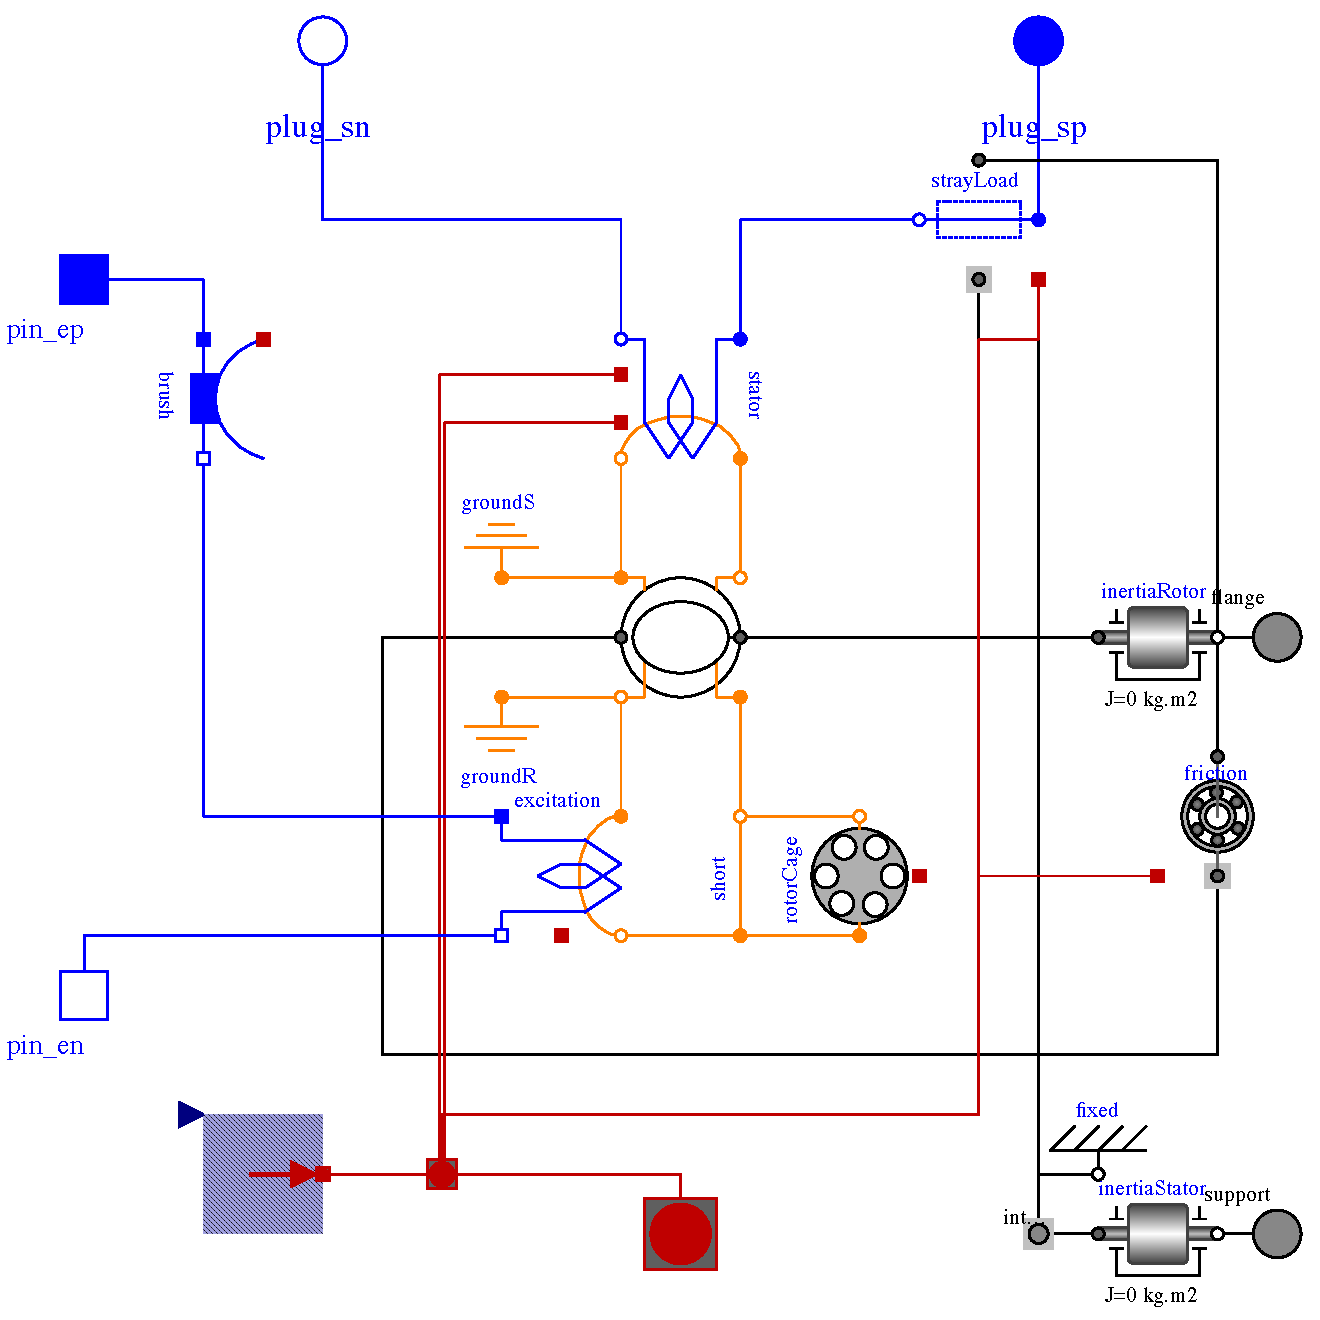
\includegraphics[height=8cm]{Bilder/SM_ElectricalExcited.pdf}
    \caption{Vollständiges Modell des elektrisch erregten Synchrongenerators mit (optionalem) Dämpferkäfig (\modclass{Fun­da­men­tal­Wave.­Ba­sic­Ma­chines.­Syn­chro­nous­In­duc­tion­Ma­chines.­SM\_­E­lec­tri­cal­Ex­ci­ted}) der MSL v3.2.3}
    \label{fig:Synchrongenerator}
\end{figure}
\cref{fig:Synchrongenerator} zeigt das vollständige Modell des elektrisch erregten Synchrongenerators mit Dämpferkäfig. Die Verwendung des Dämpferkäfigs wird über den Parameter \modclass{useDamperCage} eingestellt. Wird dieser Parameter auf \modclass{false} gesetzt, wird das Modell mit dem Verbindungsmodell \modclass{short} anstelle des Dämpferkäfigs initialisiert. 


Wie das mehrphasige Windungsmodell des Stators
berücksichtigt auch das einphasige Modell (\modclass{FundamentalWave.­Ba­sic­Ma­chines.­Com­po­nents.­Sin­gle­Phase­Win­ding}) neben der elektromagnetischen
Kopplung ohmsche Verluste und den magnetischen Streufluss.
% \begin{figure}
%     \centering
%     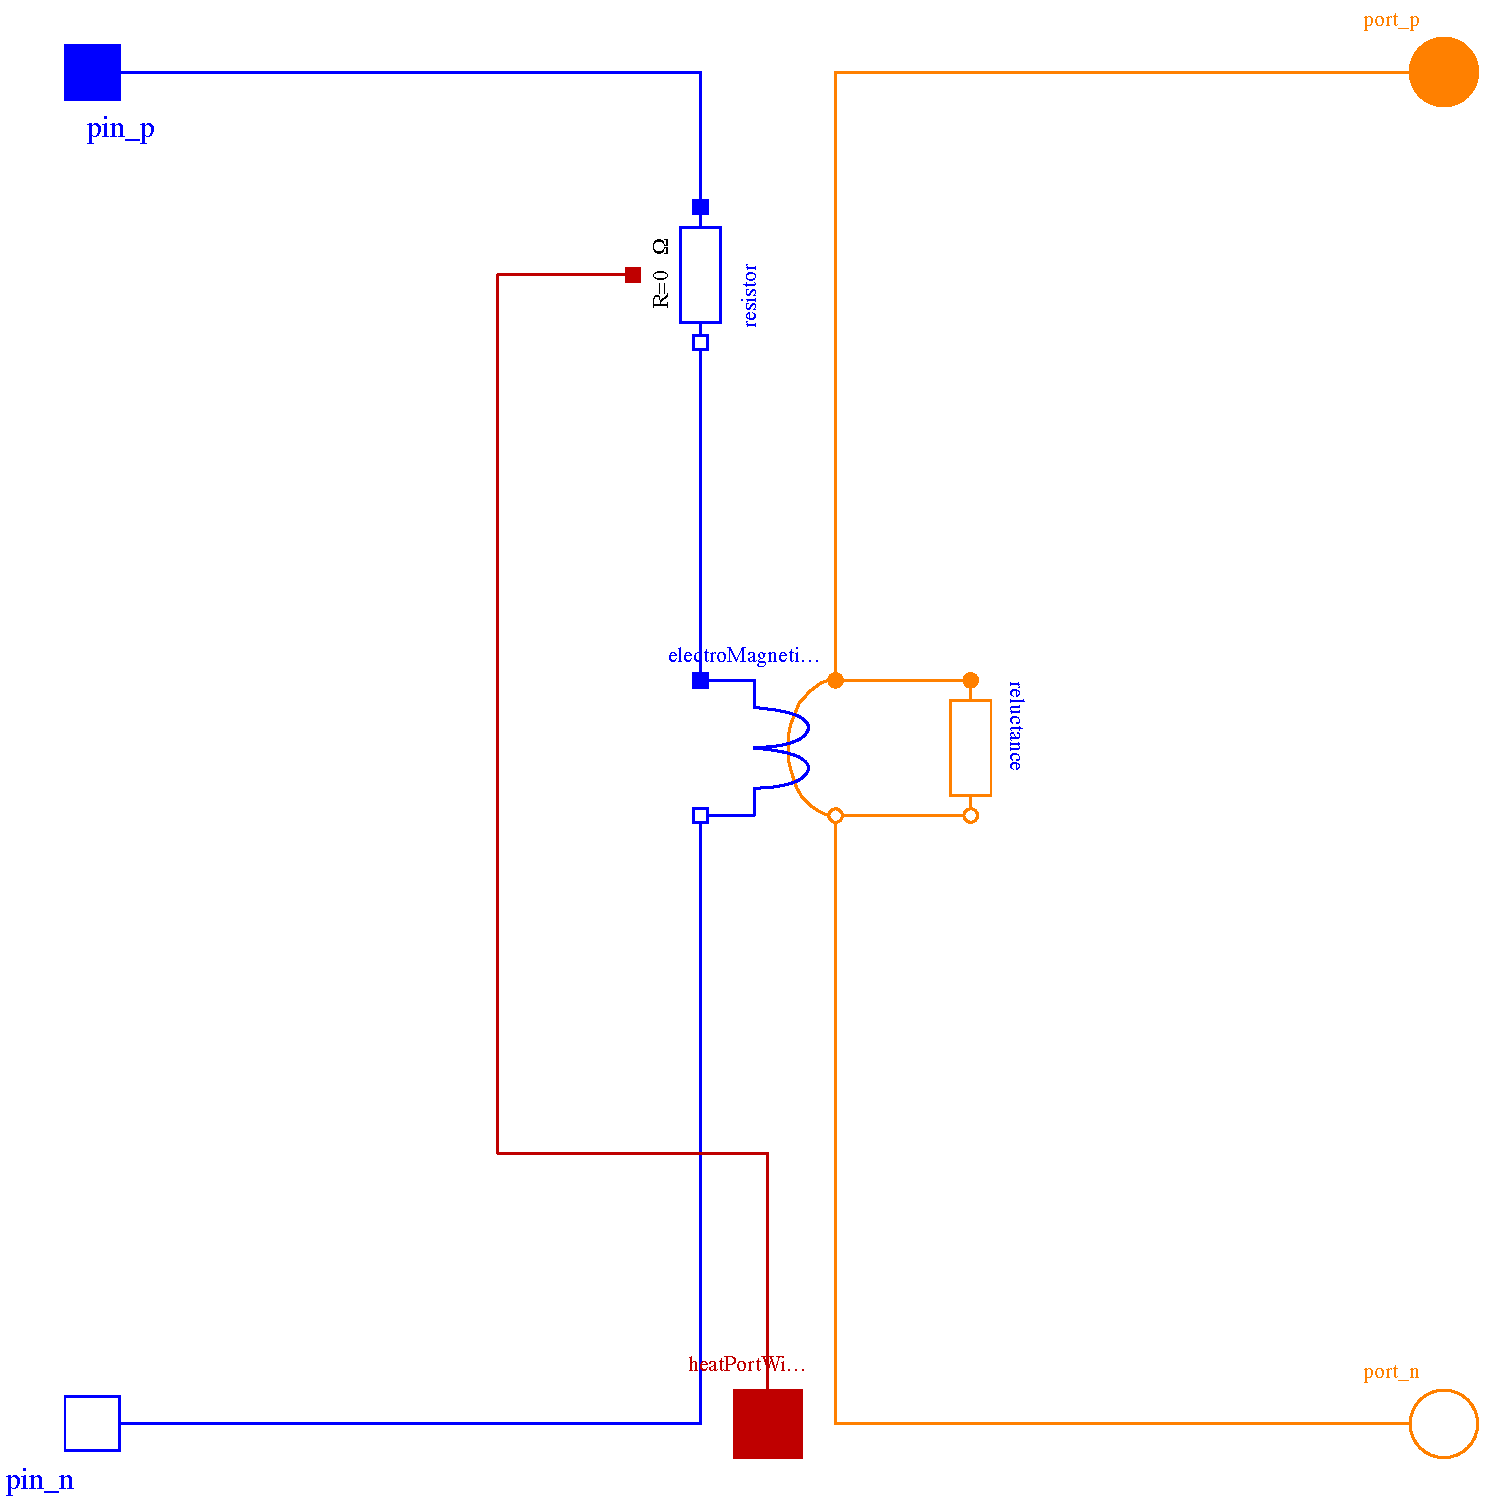
\includegraphics{Bilder/SinglePhaseWinding.pdf}
%     \caption{Einphasiges Windungsmodell (\modclass{FundamentalWave.­Ba­sic­Ma­chines.­Com­po­nents.­Sin­gle­Phase­Win­ding}) der MSL v3.2.3}
%     \label{fig:EinphasigesWicklungsmodell}
% \end{figure}

Da der Synchrongenerator über die Erregermaschine erregt wird, findet
keine Stromübertragung über Kohlebürsten statt und das Modell der
Kohlebürsten soll hier nicht beschrieben werden. Weiterhin beträgt der
Spannungsabfall über den Kohlebürsten in der Voreinstellung Null Volt.
Daher brauchen für die Kohlebürsten keine Parameter angegeben zu werden,
um einen Einfluss auszuschließen.

Das Modell des Dämpferkäfigs (\modclass{Fun­da­men­tal­Wave.­Ba­sic­Ma­chines.­Com­po­nen­ts.­Sa­li­en­cy­Cage­Win­ding}) weist die gleiche Struktur auf
wie der oben beschriebene Kurzschlussläufer. Im Unterschied zu diesem
berücksichtigt das Dämpferkäfigmodell hingegen die Achsigkeit (d- und
q-Achsen des körperfesten Koordinatensystems) der Widerstände und
Induktivitäten aufgrund der Pollücken des Dämpferkäfigs
(\cite[S. 194]{kralModelicaObjektorientierteModellbildung2019}).
Dementsprechend ist das Modell zweiphasig ausgeführt.
% \begin{figure}
%     \centering
%     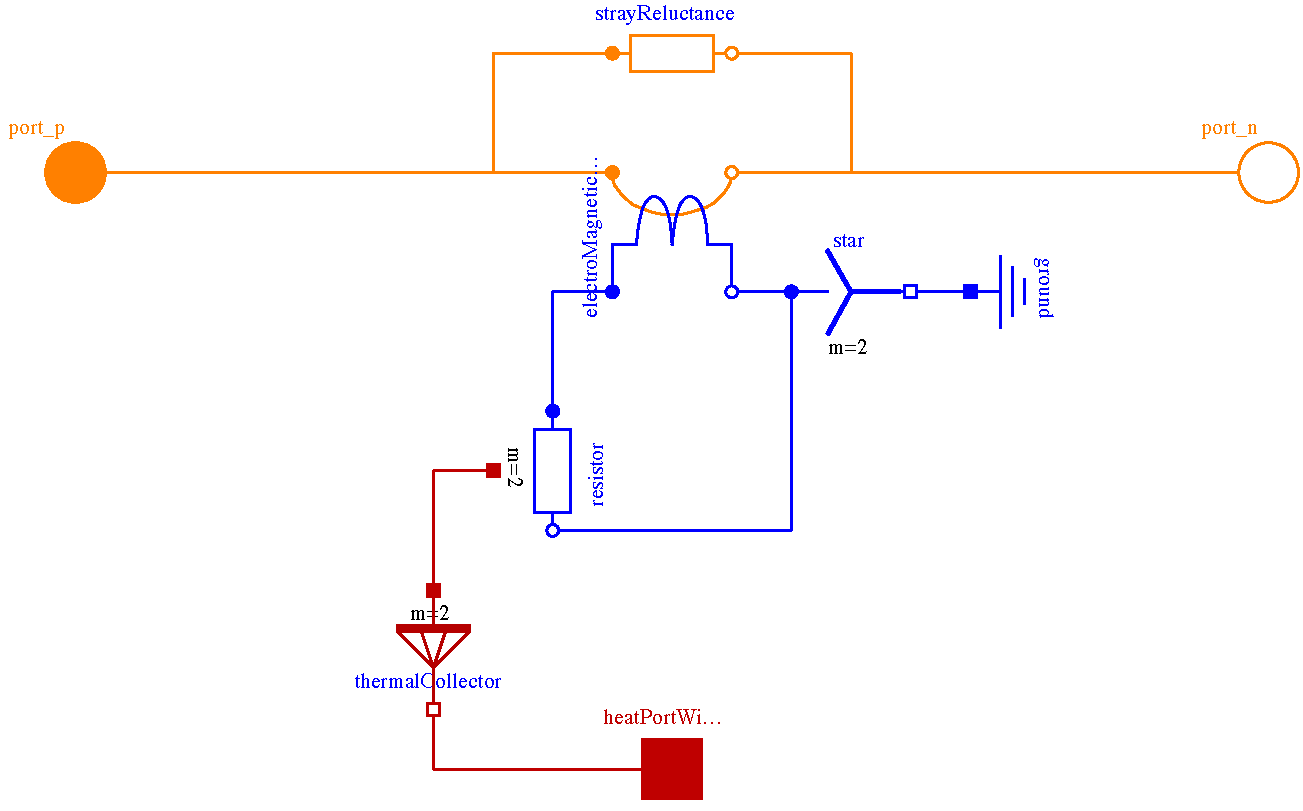
\includegraphics{Bilder/SaliencyCageWinding.pdf}
%     \caption{Caption}
%     \label{fig:SaliencyCageWinding}
% \end{figure}

\subsubsection{Parametrierung}\label{parametrierung-SG}

Alle Parameter des Synchrongenerators werden in dem Parameterrecord
\modclass{Ma­chines.­U­ti­li­ties.­Pa­ra­me­ter­Re­cords.­SM\_­E­lec­tri­cal­Ex­ci­ted­Da­ta}
der MSL v3.2.3 erfasst. Die mechanischen und thermischen Parameter des
Synchrongenerators sind dieselben wie die der Asynchronmaschine: Die
Temperaturen betragen \(\unit[20]{^\circ C}\) Umgebungstemperatur bei
Vernachlässigung der Temperaturabhängigkeit der Widerstände und das
Trägheitsmoment wird ebenfalls in dem kombinierten Trägheitsmoment des
Lüfters erfasst.

Die zur Parametrierung des Synchrongenerators verwendeten elektrischen Größen sind die im Erstzschaltbild \cref{fig:ESB_SM} angegebenen Widerstände und Induktivitäten. Aus der Auslegung der Maschine hingegen sind die in \cref{tab:AuslegungSG} aufgelisteten Größen bekannt. Die zur Umrechnung benötigten Zusammenhänge sollen im Folgenden angegeben werden. Zwar sind die hier angegebenen Zusammenhänge zum größten Teil auch in dem Parameterrecord \modclass{Machines.Utilities.SynchronousMachineData} implementiert, jedoch erfordert der Parameterrecord die Kenntnis der Ankerzeitkonstante \(T_{\mathrm{a}}\) zur Berechnung des Statorwiderstands \(R_{\mathrm{s}}\). Da jedoch \(R_{\mathrm{s}}\) (im Gegensatz zu \(T_{\mathrm{a}}\)) aus der Auslegung bekannt ist, erfolgt hier diese angepasste Umformung der Kenngrößen.

Nach \cite[S. 264]{kralModelicaObjektorientierteModellbildung2019} können die bezogenen Hauptfeldreaktanzen \(x_{\mathrm{md}}\) und \(x_{\mathrm{mq}}\) mit
\begin{align}
    x_{\mathrm{md}} &= x_{\mathrm{d}} - x_{\mathrm{s}} \\
    x_{\mathrm{mq}} &= x_{\mathrm{q}} - x_{\mathrm{s}}
\end{align}
aus den bezogenen Reaktanzen \(x_{\mathrm{d}}\) und \(x_{\mathrm{q}}\) sowie der Streureaktanz \(x_{\mathrm{s}}\) bestimmt werden. An dieser Stelle verwendet \cite[]{kralModelicaObjektorientierteModellbildung2019} anstelle von \(x_{\mathrm{s}}\) die Nullreaktanz \(x_{\mathrm{0}}\), die in etwa mit der Streureaktanz übereinstimmt. Da hier aber die Streureaktanz aus der Auslegung bekannt ist, soll \(x_{\mathrm{s}}\) direkt verwendet werden. 

Weiterhin wird dort die Reaktanz der Erregerwicklung gemäß
\begin{equation}
    x_{\mathrm{e}} = \frac{x_{\mathrm{md}}^2}{x_{\mathrm{d}}-x_{\mathrm{d}}'}
\end{equation}
angegeben. Ebenso seien die Zusammenhänge für die bezogenen Rotorreaktanzen \(x_{\mathrm{rd}}\) und \(x_{\mathrm{rq}}\)
\begin{align}
    x_{\mathrm{rd}} &= \frac{x_{\mathrm{md}}^2}{x_{\mathrm{d}}' - x_{\mathrm{d}}''}\cdot \left( 1-\frac{x_{\mathrm{md}}}{x_{\mathrm{d}}}\right)^2 + \frac{x_{\mathrm{md}}^2}{x_{\mathrm{e}}}\\
    \intertext{und}
    x_{\mathrm{rq}} &= \frac{x_{\mathrm{mq}}^2}{x_{\mathrm{q}} - x_{\mathrm{q}}''}.
\end{align}
Für die bezogenen Rotorwiderstände\footnote{An dieser Stelle liegt in der vorliegenden Ausgabe von \cite[]{kralModelicaObjektorientierteModellbildung2019} ein Druckfehler vor (vgl. mit dem \textsc{Modelica}-Code Listing \cite[S. 266]{kralModelicaObjektorientierteModellbildung2019})} wird ebenda
\begin{align}
    r_{\mathrm{rd}} &= \frac{x_{\mathrm{rd}} - \frac{x_{\mathrm{md}}^2}{x_{\mathrm{e}}}}{\omega_{\mathrm{sN}}\cdot T_{\mathrm{d0}}''}, \\
    r_{\mathrm{rq}} &= \frac{x_{\mathrm{rq}}}{T_{\mathrm{q0}}''}
\end{align}
angegeben und für den bezogenen Widerstand der Erregerwicklung
\begin{equation}
    r_{\mathrm{e}} = \frac{x_{\mathrm{e}}}{\omega_{\mathrm{sN}}\cdot T_{\mathrm{d0}}''}.
\end{equation}
Die beiden Subtransienten Leerlaufzeitkonstanten \(T_{\mathrm{d0}}''\)
und \(T_{\mathrm{q0}}''\) sind nach
\cite[S. 222ff.]{bonfertBetriebsverhaltenSynchronmaschine1962} über den Zusammenhang
\begin{align}
T_{\mathrm{d0}}'' &= \frac{x_{\mathrm{d}}'}{x_{\mathrm{d}}''}T_{\mathrm{d}}'' \\
T_{\mathrm{q0}}'' &= \frac{x_{\mathrm{q}}}{x_{\mathrm{q}}''}T_{\mathrm{q}}
\end{align}
aus den Kurzschlusszeitkonstanten \(T_{\mathrm{d}}''\) und
\(T_{\mathrm{q}}''\) berechenbar.

Damit ergeben sich die Induktivitäten und Widerstände des
Synchrongenerators mit der Nennkreisfrequenz
\(\omega_{\mathrm{sN}}=2\pi\cdot f_{\mathrm{sN}}\) und der
Bezugsreaktanz \(X_{\mathrm{N}}\) nach \cref{eq:LmgSG,eq:ReSG} (vgl.
\cite[S.265f.]{kralModelicaObjektorientierteModellbildung2019}).
\begin{align}
L_{\mathrm{md}} &= x_{\mathrm{md}}\cdot \frac{X_{\mathrm{N}}}{\omega_{\mathrm{sN}}} \label{eq:LmgSG}\\
L_{\mathrm{mq}} &= x_{\mathrm{mq}}\cdot \frac{X_{\mathrm{N}}}{\omega_{\mathrm{sN}}} \\
L_{\mathrm{r \sigma d}} &= (x_{\mathrm{rq}}-x_{\mathrm{mq}})\cdot \frac{X_{\mathrm{N}}}{\omega_{\mathrm{sN}}} \\
L_{\mathrm{r \sigma q}} &= (x_{\mathrm{rd}}-x_{\mathrm{md}})\cdot \frac{X_{\mathrm{N}}}{\omega_{\mathrm{sN}}} \\
L_{\mathrm{s \sigma}} &= x_{\mathrm{s}}\cdot \frac{X_{\mathrm{N}}}{\omega_{\mathrm{sN}}} \\
R_{\mathrm{rd}} &= r_{\mathrm{rd}}\cdot X_{\mathrm{N}} \\
R_{\mathrm{rq}} &= r_{\mathrm{rq}}\cdot X_{\mathrm{N}} \\
R_{\mathrm{e}} &= \frac{3}{2}\cdot \left(\frac{\sqrt{2}U_{\mathrm{sNenn}}}{\omega_{\mathrm{sN}}L_{\mathrm{md}}\cdot I_{\mathrm{Err. Leerl.}}}\right)^2\cdot r_{\mathrm{e}}\cdot X_{\mathrm{N}}\label{eq:ReSG}
\end{align}
Damit ist der Synchrongenerator vollständig parametriert. Die \cref{tab:AuslegungSG,tab:ZwischenwerteSG,tab:ParameterRecordSG,tab:ParameterSG} listen eine Übersicht über alle Parameter und Berechnungsgrößen auf.

\subsection{Erregermaschine}\label{sec:erregermaschine}

Die Erregermaschine und der auf dem Polrad der Maschine mitrotierende Gleichrichter dienen gemäß \cref{fig:Wirkungsgraph} der berührungslosen Erregung des Synchrongenerators über den Luftspalt. Wie bei dem Hauptgenerator handelt es sich auch bei der Erregermaschine um eine Synchronmaschine. Neben der geringeren Größe (ermöglicht durch die geringere Übertragungsleistung) unterscheiden sich die beiden Generatoren darin, dass die Erregermaschine eine Innenpol- und der Hauptgenerator eine Außenpolmaschine ist. In dem zu modellierenden Verhalten der Maschinen tritt dieser Unterschied jedoch nicht auf und braucht daher nicht berücksichtigt zu werden.

\subsubsection{Modell}\label{modell-erregermaschine}

\cref{fig:Erregermaschine} zeigt das vollständige Modell der in der \modclass{Frequenzumformer}-Bibliothek implementierten Erregermaschine. Als Generatormodell wird dasselbe Synchrongeneratormodell der MSL wie für den Hauptgenerator verwendet. Das \modclass{delta}-Modell zwischen den beiden dreiphasigen Ausgängen des Generators bewirkt eine Verkettung der Ströme und Spannungen wie in einer Dreieckschaltung der Statorstränge.

Die Gleichrichtung der erzeugten dreiphasigen Spannung geschieht mit einem 6-Puls-Brückengleichrichter. Am negativen Ausgang des Brückengleichrichters wird ein (\unit[0]{V}) Referenzpotential verschaltet, ohne das die Gleichungen für den elektrischen Kreis zwischen Erregermaschine und Synchrongenerator nicht eindeutig lösbar wären.

Die Dioden des Gleichrichter verwenden ein ideales Diodenmodell mit zwei linearen Arbeitsbereichen \emph{Sperrbetrieb} und \emph{Durchlassbetrieb}. Die Steigung der Diodenkennlinien in den beiden Arbeitsbereichen wird über den Leitwert \(G_{\mathrm{off}}\) im Sperrbetrieb und den Widerstand \(R_{\mathrm{on}}\) im Durchlassbetrieb eingestellt. Der Wechsel vom Sperrbetrieb in den Durchlassbetrieb findet bei Überschreiten der Flussspannung \(U_{\mathrm{F}}\) statt. Ebenso wird zurück in den Sperrbetrieb geschaltet, sobald die Flussspannung unterschritten wird.

\begin{figure}
    \centering
    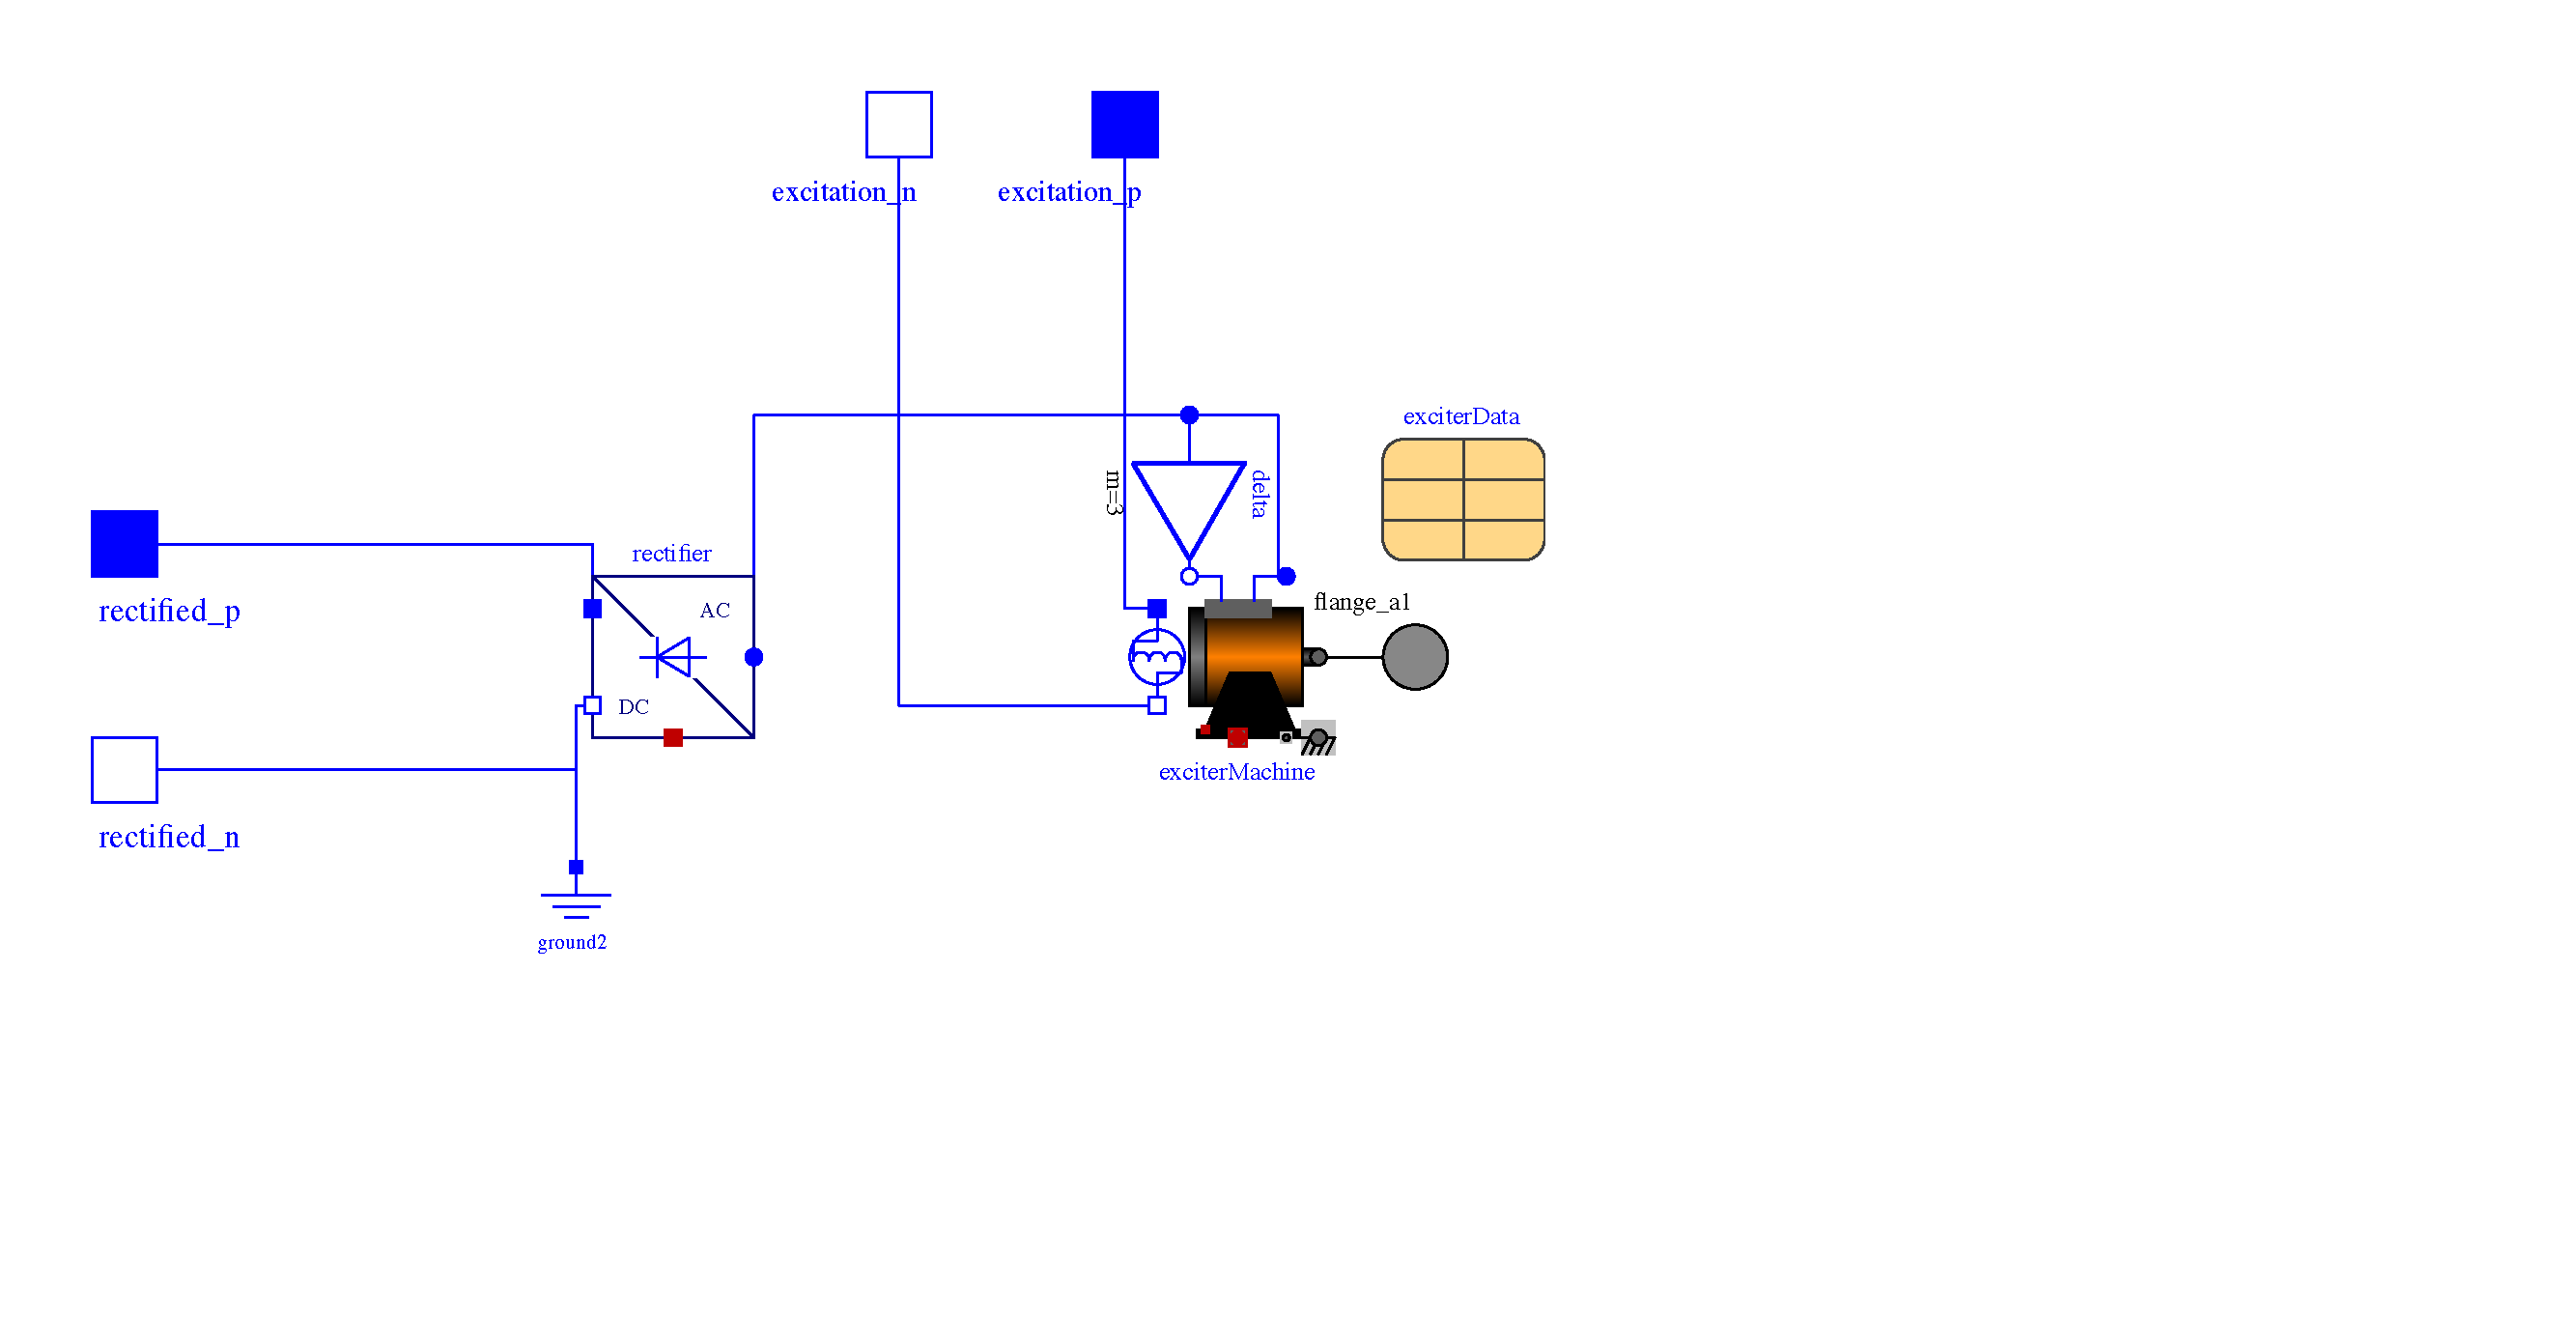
\includegraphics[height=6cm]{Bilder/SM_Erreger.pdf}
    \caption{Vollständiges Modell der Erregermaschine}
    \label{fig:Erregermaschine}
\end{figure}

% \begin{figure}
%     \centering
%     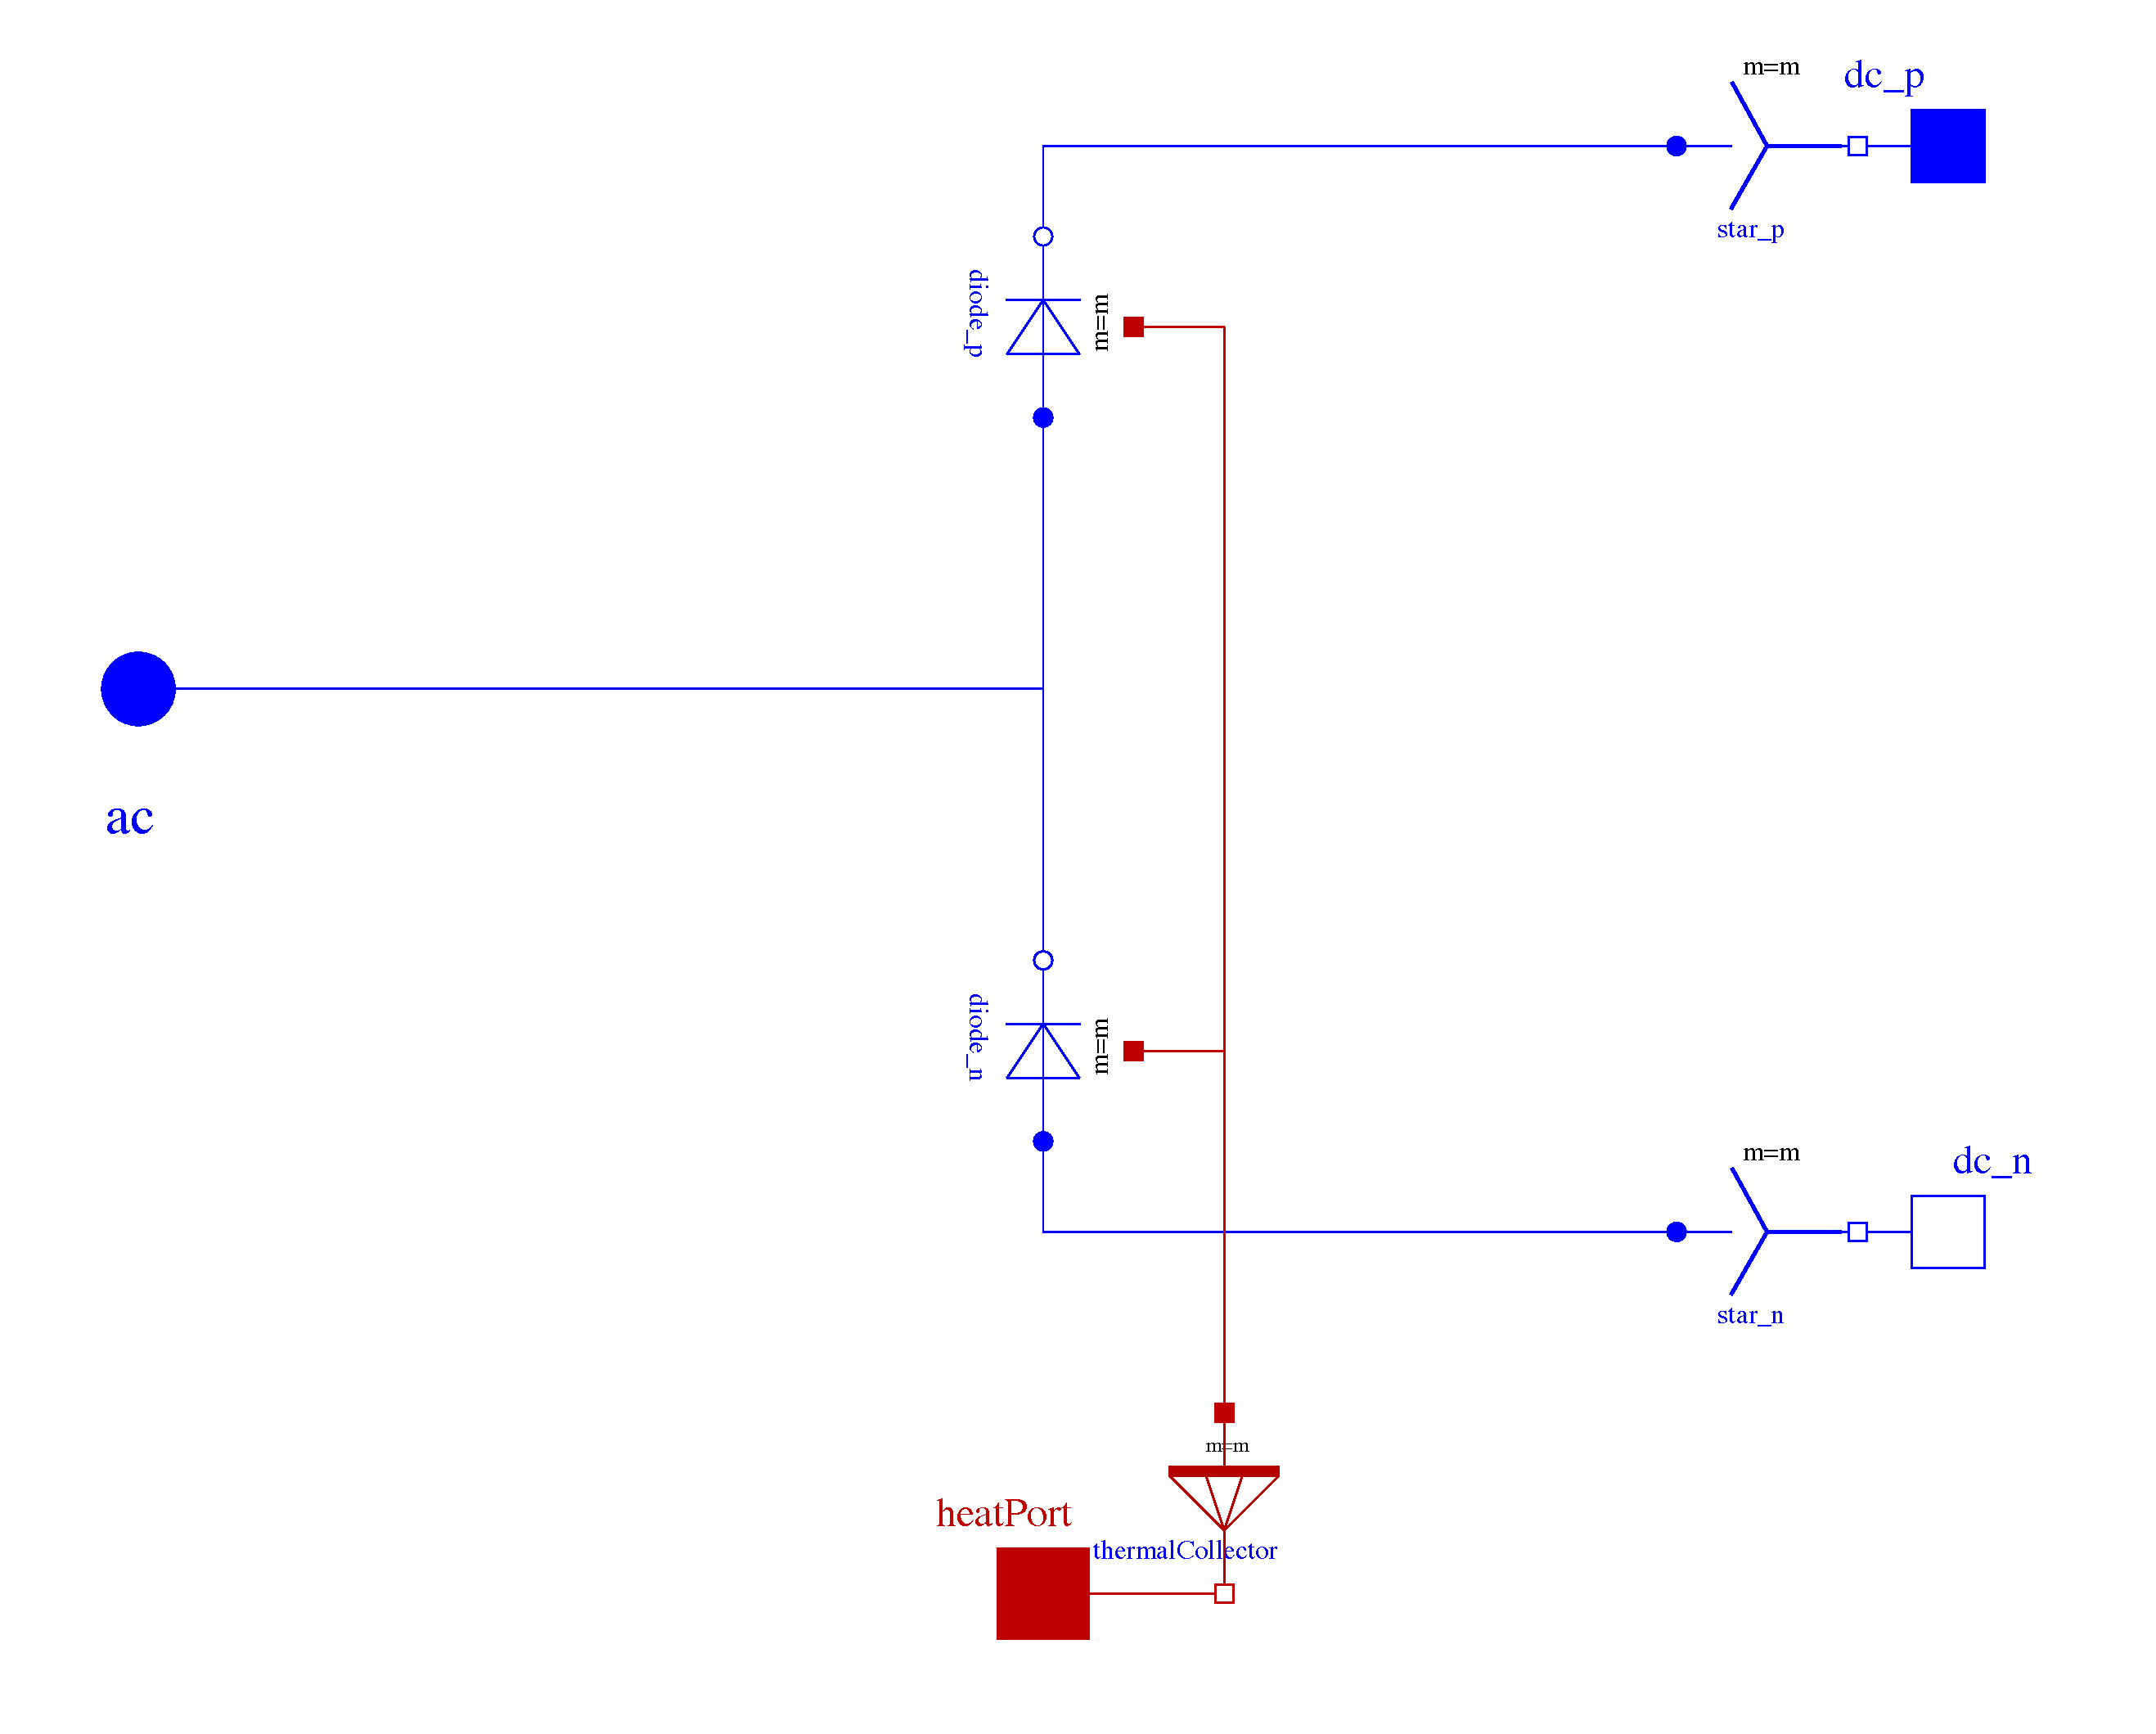
\includegraphics{Bilder/DiodeBridge2mPulse.pdf}
%     \caption{Vollständiges Modell des Dioden-Gleichrichters}
%     \label{fig:Gleichrichter}
% \end{figure}

\hypertarget{parametrierung-2}{%
\subsubsection{Parametrierung}\label{parametrierung-2}}

Die Parametrierung des Synchrongenerators der Erregermaschine erfolgt
analog zur Parametrierung des Hauptgenerators oben. Die verwendeten
Größen sind in  \cref{tab:AuslegungErregermaschine,tab:ParameterErregermaschine,tab:ParameterRecordErregermaschine,tab:ZwischenwerteErregermaschine} dargestellt.

Für den Brückengleichrichter sind aus der Auslegung keine Werte bekannt. Daher wird für die Flussspannung \(U_{\mathrm{F}}=\unit[0,7]{V}\) (typischer Wert für Silizium-Dioden \cite{??} ) angenommen. Der Leitwert \(G_{\mathrm{off}}\) und der Widerstand \(R_{\mathrm{on}}\) einer idealen Diode betragen Null. Um jedoch numerische Probleme (Teilen durch Null bzw. Ansteigen der resultierenden Größen gegen Unendlich) zu vermeiden, werden \(G_{\mathrm{off}}=\unit[0,001]{S}\) bzw. \(R_{\mathrm{on}}=\unit[0,001]{\Omega}\) festgelegt, die nahe Null, aber noch groß genug sind um die genannten Probleme zu vermeiden.

\subsection{Spannungsregler}\label{sec:Spannungsregler}
Der Spannungsregler wird in \textsc{Modelica} als Signalflussobjekt implementiert. Zur Unterstützung des objektorientierten Ansatzes werden die Teilglieder des Reglers (P-Glied, I-Glied und D-Glied) als eigenständige Objekte definiert, die in dem Spannungreglermodell verwendet werden.

Wie im Blockschaltbild des Reglers (\cref{fig:Blockschaltbild_Regler}) dargestellt, ist allen Regelgliedern ein Begrenzer nachgeschaltet. Dies trägt zum Einen der Abbildung der Messgrößen auf das begrenzte Intervall der reglerinternen Größen Rechnung und bietet zum Anderen die Möglichkeit, die Stellgrößen der Regelglieder unabhängig voneinander zu begrenzen. Um diese Begrenzung bei allen Gliedern mit einer einheitlichen Schnittstelle zu implementieren wird aus dem \textbf{S}ingle-\textbf{I}nput-\textbf{S}ingle-\textbf{O}utput-Interface der MSL (\modclass{Mo­de­li­ca.­Blocks.­In­ter­fa­ces.­SI­SO}) das Interface \modclass{Frequenzumformer.Regler.Interfaces.limitedController} abgeleitet, welches die Begrenzungsgrößen zugänglich macht. Weiterhin wird in dem Interface der boolsche Eingang \modclass{enable} definiert zum Einschalten des jeweiligen Regelgliedes.­

\paragraph{Modell}\label{modell-Regler}
Das vollständige Modell des Spannungsreglers zeigt \cref{fig:Spannungsregler-Modell}. Es enthält die drei Teilglieder des PID-Reglers, die Stellgrößenbeschränkung und am Ausgang einen Schalter um den Wert Null auszugeben, wenn der Regler ausgeschaltet ist. Die Modelle der drei Teilregler zeigen die \cref{fig:D-Regler,fig:P-Regler,fig:I-Regler}. Das Modell des P-Reglers bietet in Anlehnung an \cite{DigitalerSpannungsreglerSoftwaredokumentation} zwei konditionale Parameter: Mit einem Schalter kann bestimmt werden, ob die Verstärkung konstant oder variabel sein soll und mit dem zweiten Schalter kann bestimmt werden, ob der Reglerausgang begrenzt werden solll. Die Simulation des Reglers erfolgt zeitkontinuierlich ohne Berücksichtigung eines Abtast-Halteglieds. Der Vergleich des implementierten Reglers mit einem zeitdiskreten Regler und einem kontinuierlichen Reglers mit Abtastglied zeigt keine nennenswerten Unterschiede in den Ergebnissen; die Simulationen mit dem diskreten Regler und mit der Abtastung benötigen jedoch die 1,5-fache Simulationszeit (Auf dem hier verwendeten Simulationssystem mit dem Solver \texttt{dassl}: zeitdiskret: $\unit[279,369]{s}$, kontinuierlich mit Abtastung: $\unit[277,589]{s}$, kontinuierlich ohne Abtastung: $\unit[182,312]{s}$). Ursache für die größere Simulationszeit ist die Begrenzung der Schrittweite des Solvers durch die \texttt{timeEvents}, die die Diskretisierung verursacht. Ohne die Diskretisierung kann die Schrittweitensteuerung des Solvers auch zwischen zwei Abtastpunkten größere Schrittweiten einstellen.
\begin{figure}
    \centering
    \begin{subfigure}{.49\textwidth}
	    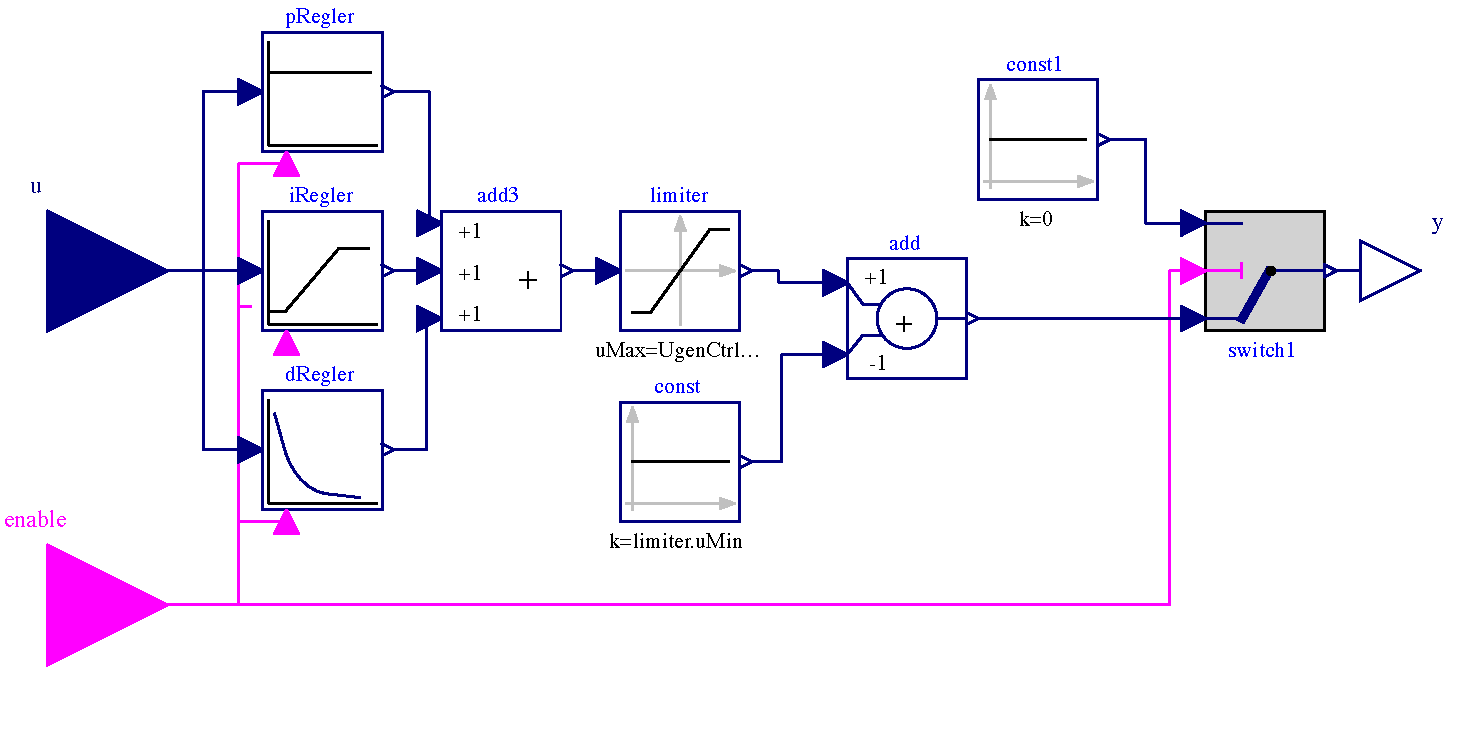
\includegraphics{Bilder/Spannungsregler.pdf}
		\caption{Vollständiges Modell des Spannungsreglers (\modclass{Fre­quenz­um­for­mer.­Reg­ler.­Span­nungs­reg­ler})}
		\label{fig:Spannungsregler-Modell}    	
    \end{subfigure}
    \begin{subfigure}{.49\textwidth}
		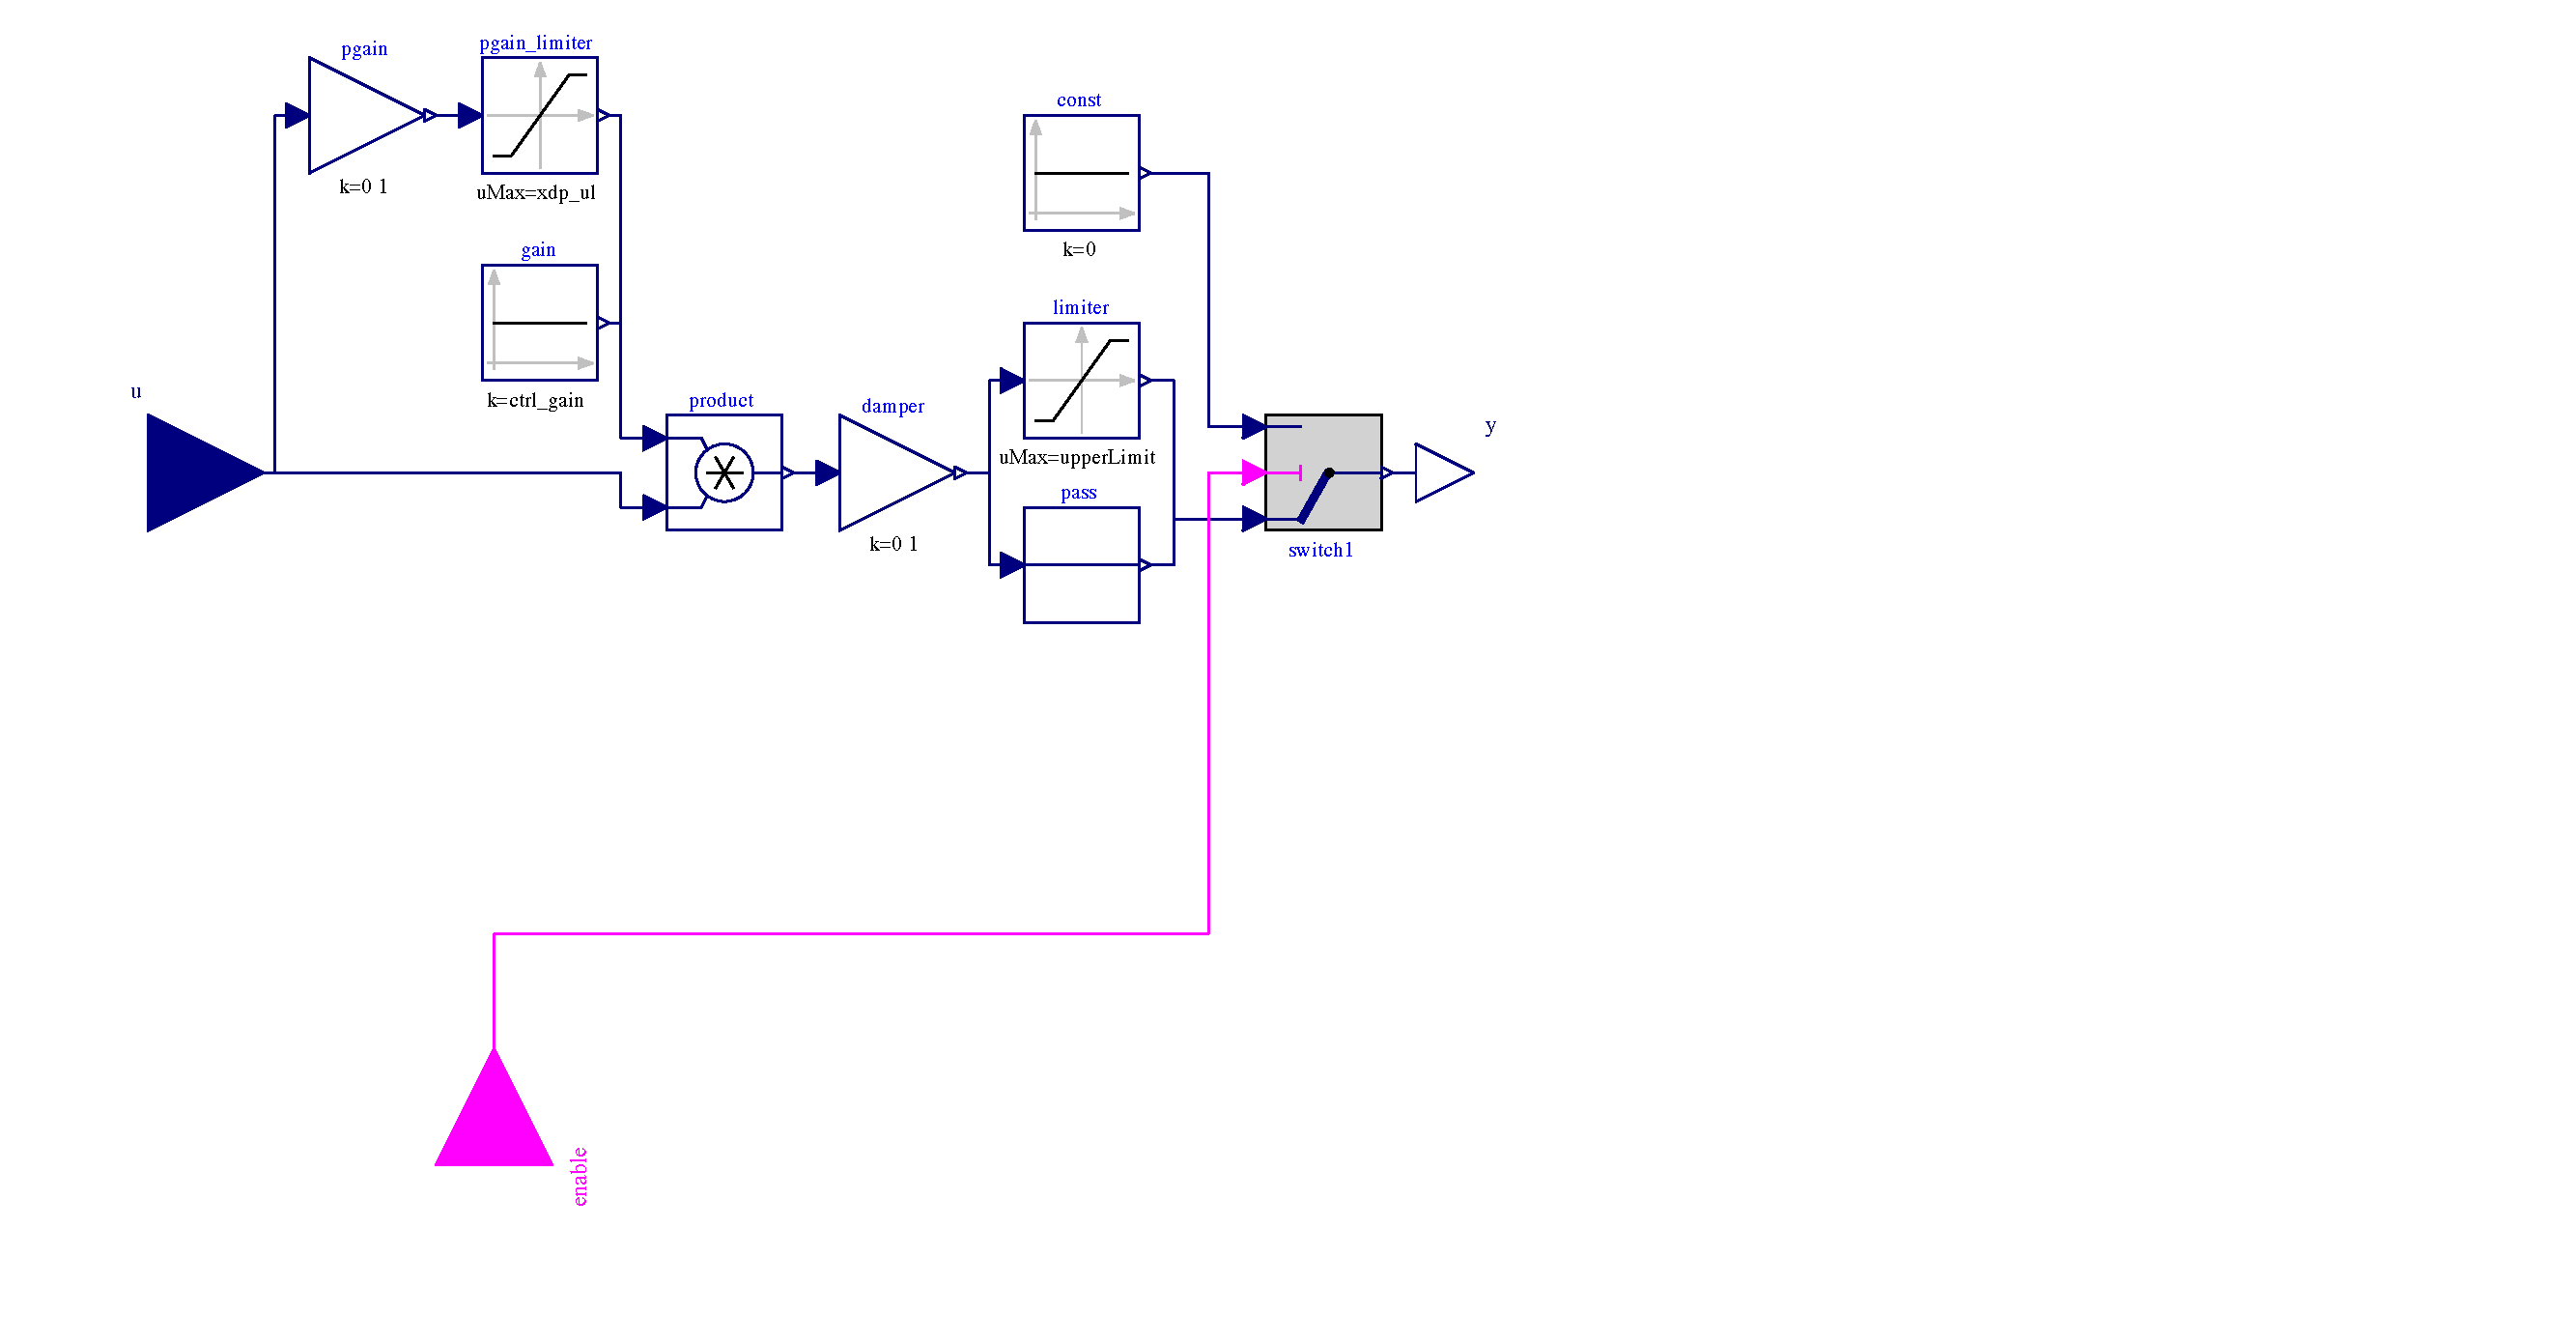
\includegraphics{Bilder/PRegler.pdf}
		\caption{Modell des Proportional-Reglers (\modclass{Fre­quenz­um­for­mer.­Reg­ler.­Kon­ti­nu­ier­lich.­PRegler})}
		\label{fig:P-Regler}
    \end{subfigure}
    \begin{subfigure}{.49\textwidth}
		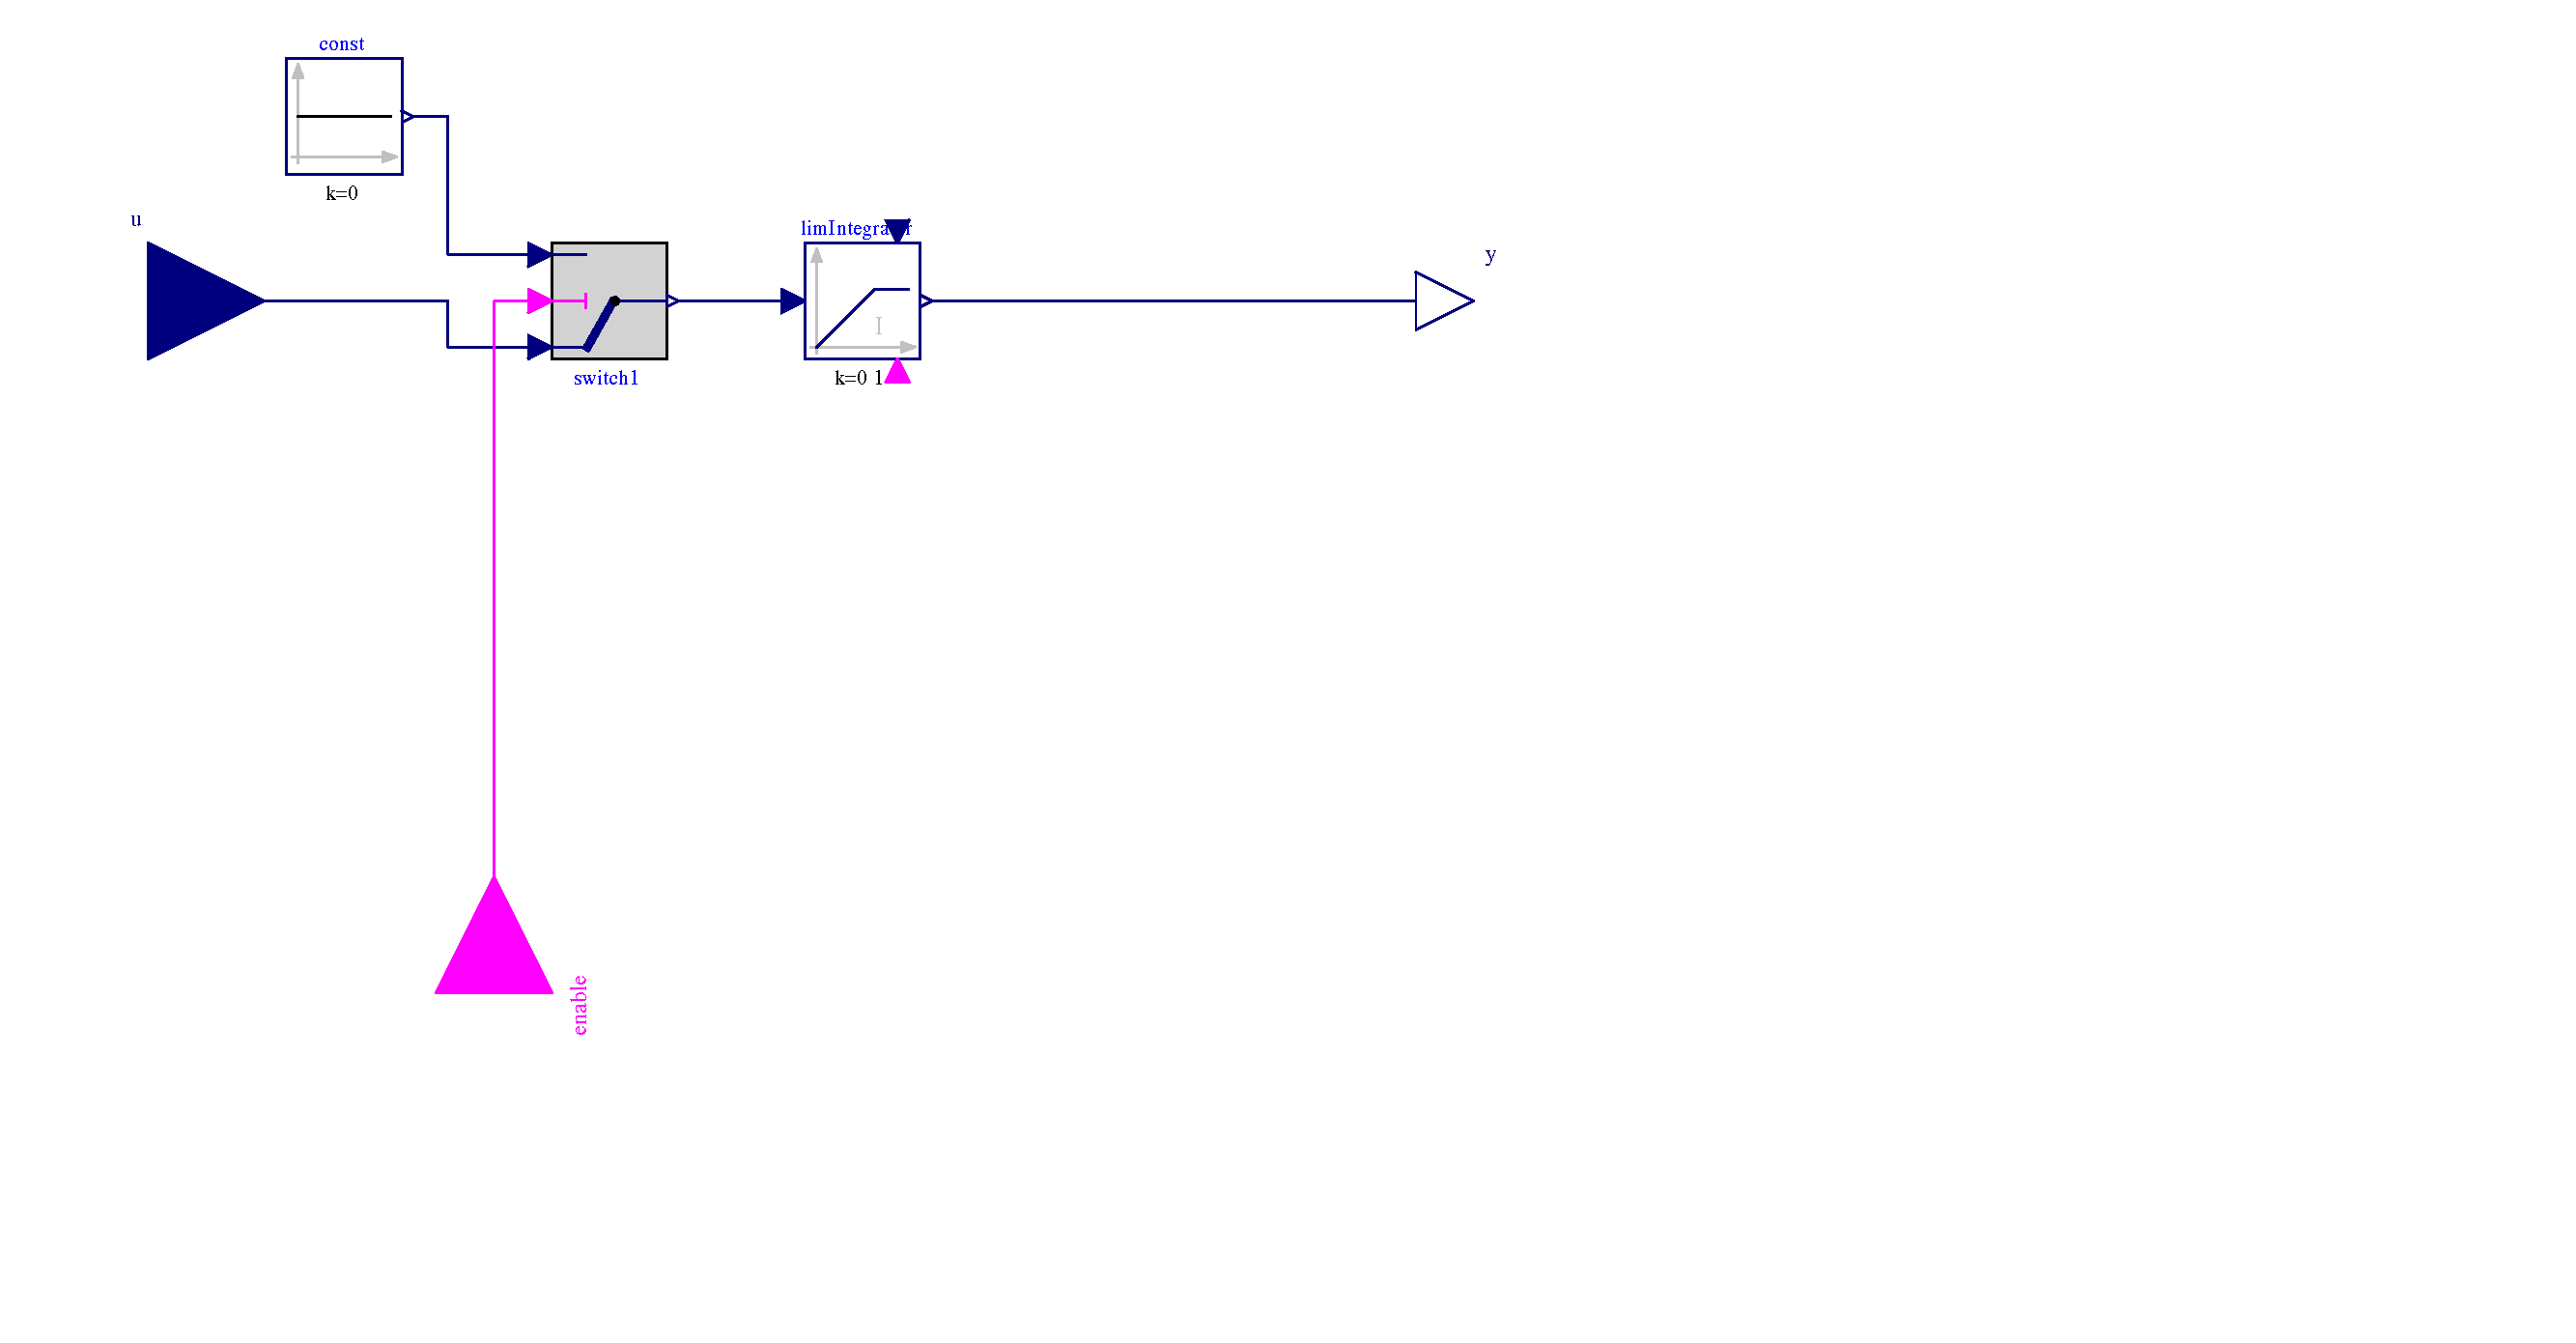
\includegraphics{Bilder/IRegler.pdf}
		\caption{Modell des I-Reglers (\modclass{Fre­quenz­um­for­mer.­Reg­ler.­Kon­ti­nu­ier­lich.­IRegler})}
		\label{fig:I-Regler}    	
    \end{subfigure}
    \begin{subfigure}{.49\textwidth}
	    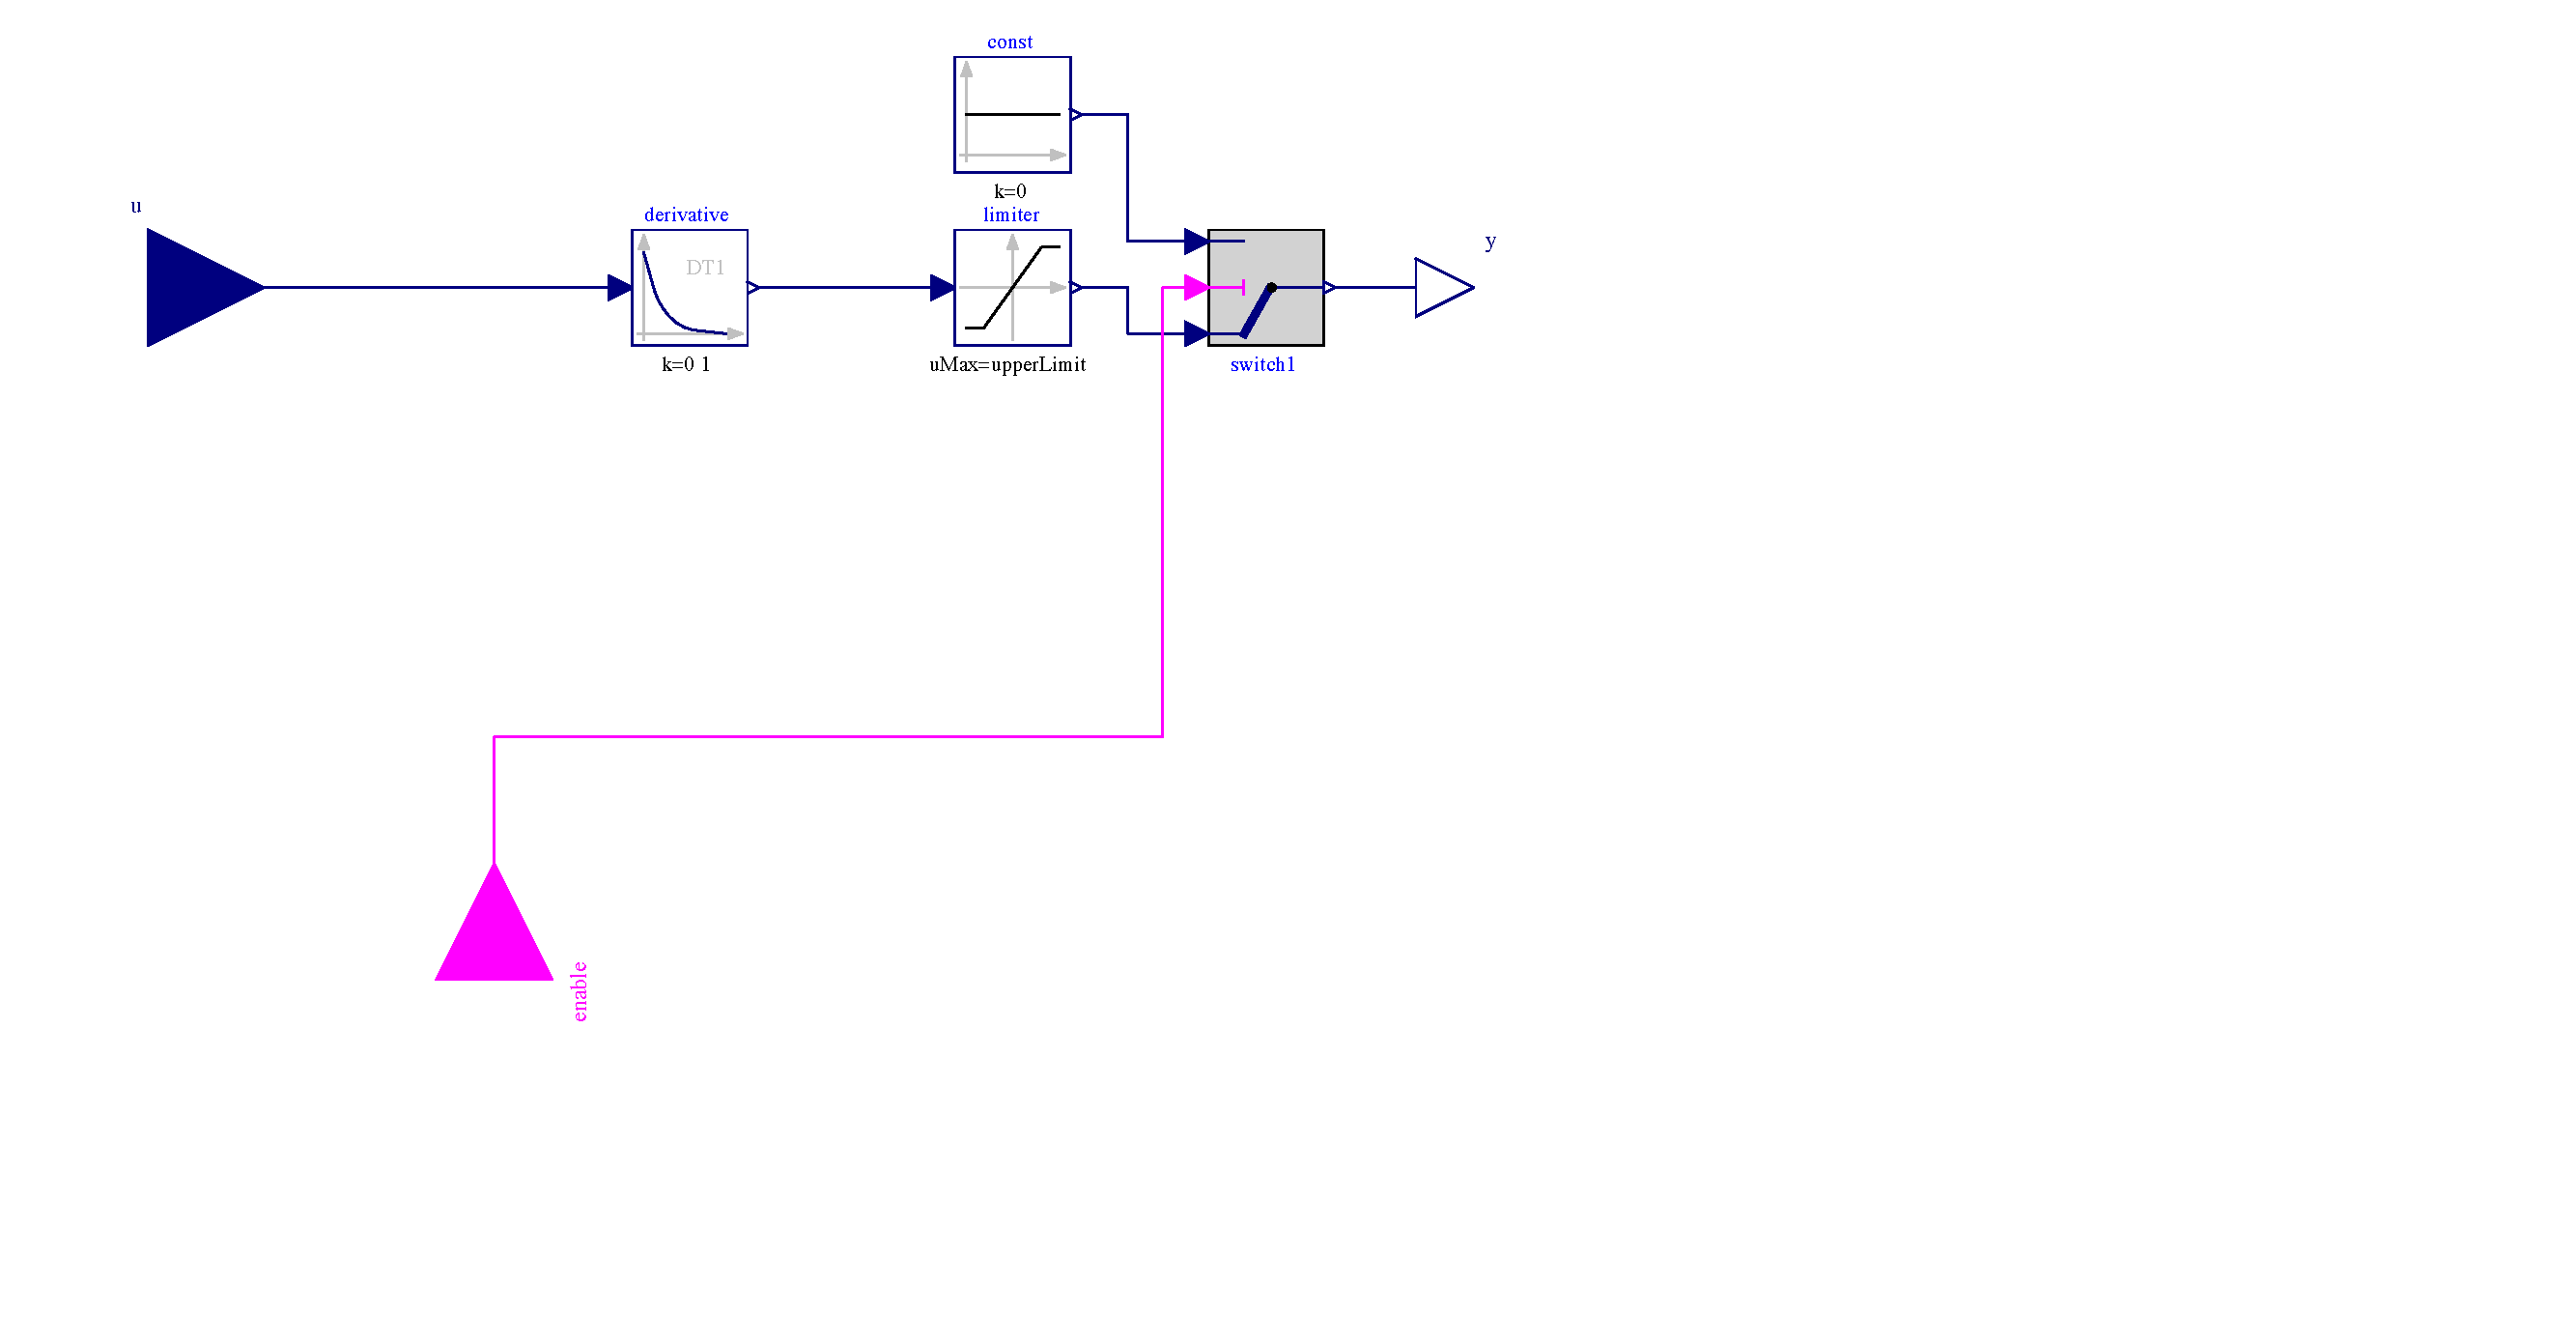
\includegraphics[]{Bilder/DRegler.pdf}
	    \caption{Modell des D-Reglers (\modclass{Fre­quenz­um­for­mer.­Reg­ler.­Kon­ti­nu­ier­lich.­DRegler})}
	    \label{fig:D-Regler}    	
    \end{subfigure}
    \caption{Modelle des Spannungsreglers und der Teilregler}
\end{figure}

\paragraph{Parametrierung} Für den Spannungsregler sollen die Reglerparameter verwendet werden, die auch bei dem realen Frequenzumformer zum Einsatz kommen. Dazu müssen die Parameter der zeitdiskreten I- und D-Glieder umgerechnet werden auf die hier simulierten kontinuierlichen Glieder. Für das diskrete I-Glied ist in \cite{piller_power_systems_piller_nodate} das Blockschaltbild des eingesetzten Reglers angegeben, mit der $\mathcal{Z}$-Übertragungsfunktion \cref{eq:ZIPiller} und den Parametern $k_\mathrm{v}$ Verstärkung und $k_\mathrm{d}$ Dämpfung des Signals.
\begin{equation}
	\label{eq:ZIPiller}
	G(z) = \frac{k_\mathrm{v}}{k_\mathrm{d}}\cdot\frac{z}{z-1}
\end{equation}
Das kontinuierliche I-Glied wird mit \cref{eq:SI} beschrieben. Nach \cref{par:ZeitdiskreterRegler} ergibt sich die $\mathcal{Z}$-Übertragungsfunktion bei Abtastung mit einem ZOH-Glied der Abtastrate $T_\mathrm{s}$ zu \cref{eq:ZI}.
\begin{align}
	G(s) &= \frac{K_\mathrm{I}}{s} \label{eq:SI}\\
	G(z) &= \frac{z-1}{z} \mathcal{Z}\left\{ \mathcal{L}^{-1}\left.\left\{\frac{G(s)}{s}\right\}\right|_{kT_{\mathrm{s}}} \right\} = K_\mathrm{I}T_\mathrm{s}\cdot\frac{z}{z-1} \label{eq:ZI}
\end{align}
Über einen Koeefizientenvergleich ergibt sich \cref{eq:IUmrechnung} zur Umrechnung der Parameter des I-Glieds.
\begin{equation}
	K_\mathrm{I} = \frac{1}{T_\mathrm{s}}\frac{k_\mathrm{v}}{k_\mathrm{d}}\label{eq:IUmrechnung}
\end{equation}
Analog ergibt sich ein Ausdruck für das D-Glied: Implementiert ist ein DT1-Glied mit der $\mathcal{Z}$-Übertragungsfunktion \cref{eq:ZDPiller} (vgl. Blockschaltbild \cite{piller_power_systems_piller_nodate}) und den Parametern Verstärkung $k_\mathrm{v}$, Dämpfung $k_\mathrm{d}$ und der Zeitkonstante $T$. Die Zeitkonstante wird auf die interne Konstante $c$ bezogen, das Maximum der reglerinternen Zahlen.
\begin{equation}
	G(z) = \frac{k_\mathrm{v}}{k_\mathrm{d}}\cdot\frac{z-1}{z-(1-\frac{T}{c})}\label{eq:ZDPiller}
\end{equation}
Aus der kontinuierlichen Übertragungsfunktion wird wieder die Übertragungsfunktion des diskreten Reglers bestimmt 
\begin{align}
	G(s) &= \frac{K_\mathrm{D}s}{T_\mathrm{D}s+1}\label{eq:SD}\\
	G(z) &= \frac{z-1}{z} \mathcal{Z}\left\{ \mathcal{L}^{-1}\left.\left\{\frac{G(s)}{s}\right\}\right|_{kT_{\mathrm{s}}} \right\} = \frac{K_\mathrm{D}}{T_\mathrm{D}}\cdot\frac{z}{z-e^{-\nicefrac{T_\mathrm{s}}{T_\mathrm{D}}}}\label{eq:ZD}
\end{align}
und über einen Koeffizientenvergleich ergeben sich \cref{eq:DKUmrechnung,eq:DTUmrechnung} für die Parameter des D-Glieds.
\begin{align}
	T_\mathrm{D} &= \frac{T_\mathrm{s}}{\ln(\frac{T}{c})}\label{eq:DTUmrechnung}\\
	K_\mathrm{D} &= T_\mathrm{D}\cdot\frac{k_\mathrm{v}}{k_\mathrm{d}}\label{eq:DKUmrechnung}
\end{align}
Diese Umrechnung wird im Modell des Spannungsreglers implementiert, sodass der Regler mit den diskreten Reglerparametern eingestellt werden kann. Die verwendeten Reglerparameter sind in \cref{sec:Reglerparameter} aufgelistet.

\subsection{Weitere Modelle}\label{sec:WeitereModelle}
Im Folgenden werden noch einige weitere Modelle geschildert, die zur Simulation des Umformers benötigt werden, aber von untergeordneter Bedeutung sind.

\paragraph{Abbildung auf reglerinterne Zahlen}
\label{sec:AbbildungReglerZahlen}
Neben der Umrechnung der Reglerparameter muss zur Simulation des Spannungsreglers auch eine Transformation des Messsignals in die reglerinternen Zahlen erfolgen. Ebenso muss das Ausgangssignal des Reglers von dem reglerinternen Wertebereich in die Stellspannung umgewandelt werden. Dies erfolgt mit dem Modell \modclass{Frequenzumformer.Regler.­Off­set\_Map}. Das Modelle rechnet die Eingabedaten mittels einer linearen Funktion um. Parametriert wird die lineare Funktion über die zwei Punkte $(I_1,O_1),\,(I_2,O_2)$ auf der Geraden. Der Umrechnungsfaktor für den Reglereingang ergibt sich aus den Parametern des eingesetzten Messtrafos und des AD-Wandlers zu
\begin{equation}
	U_\mathrm{intern} = U_\mathrm{real}\cdot 15,1875.
\end{equation}
Die Erzeugung der Erregerspannung erfolgt am realen Umformer mittels eines Steuertrafos und Puls-Weiten-Modulation. Im Simulationsmodell wird diese Umsetzung vereinfacht. Über das \modclass{Offset\_Map}-Modell wird direkt die Erregerspannung aus der Stellgröße des Reglers berechnet. Der Spannungsregler kann Puls-Weiten im Intervall $[0,32767]$ einstellen. Diese werden abgebildet auf den Spannungsbereich des Steuertrafos im Intervall $[\unit[0]{V},\unit[80]{V}]$. %Dieser Spannungsbereich des Steuertrafos ist jedoch mit einer Unsicherheit behaftet. Eine Datenquelle gibt auch einen möglichen Bereich bis \unit[120]{V} an.

\paragraph{Leistungsmessung}\label{leistungsmessung}
Zur Leistungsmessung wurde das Modell \modclass{E­lec­tri­cal.­Ma­chines.­Sen­sors.­E­lec­tri­cal­Po­wer­Sen­sor}­ der MSL erweitert, sodass auch Scheinleistung und Wirkfaktor aus der Wirk- und der Blindleistung bestimmt werden können. Da der eingesetzte Sensor Wirk- und Blindleistung aus einer Raumzeigertransformation der dreiphasigen Spannung bestimmt, ist die Leistungsmessung nur zuverlässig, wenn in der Simulation an der in Stern geschalteten Last kein Rückleiter angeschlossen wird.

\paragraph{Modellierung der Last}\label{parametrierung-der-last}
Die Belastung des Frequenzumformers wird in der Simulation durch die Reihenschaltung eines variablen Widerstands und einer variablen Induktivität in Sternschaltung modelliert. Über eine zeitgesteuerte Tabelle können so verschiedene Laststufen und Lastsprünge eingestellt werden. Berechnet werden die Lastgrößen aus der Nennscheinleistung, der Nennspannung und dem gewünschten Wirkfaktor. Für \unit[100]{\%} Last ergibt sich beispielsweise:
\begin{align}
Z_{100\%} &= 3\cdot\frac{U_{Nenn}^2}{S_{Nenn}}= 3\cdot \frac{\unit[115]{V^2}}{\unit[90]{kVA}} = \unit[0,44083]{\Omega} \\
R_{100\%} &= \sqrt{\frac{Z^2}{1+\tan^2(\arccos(\cos\varphi))}}=\sqrt{\frac{(\unit[0,44083]{\Omega})^2}{1+\tan^2(\arccos(0,8))}}=\unit[0,352664]{\Omega} \\
X_{100\%} &= \sqrt{Z^2-R^2}=\sqrt{(\unit[0,44083]{\Omega})^2 - (\unit[0,352664]{\Omega})^2}=\unit[0,264498]{\Omega} \\
\intertext{Mit $f=\unit[400]{Hz}$:}
L_{100\%} &= \frac X\omega = \frac{\unit[0,264498]{\Omega}}{2\pi\cdot\unit[400]{Hz}}\approx \unit[105,24]{mH}\\
\end{align}

\paragraph{Messung der Frequenz}
Da die direkte Messung der Spannungsfrequenz (z.B. durch Messen der Zeit zwischen Nulldurchgängen oder mittels Fouriertransformation) numerisch sehr aufwendig ist, wird die Spannungsfrequenz aus der Winkelgeschwindigkeit der rotierenden Masse bestimmt. In \textsc{Modelica} ist die Winkelgeschwindigkeit  als Flussgröße der rotatorischen Mechanik festgelegt und daher eine Zustandsgröße, die direkt ausgelesen und verarbeitet werden kann. Die Frequenz der Spannung ergibt sich dann aus der Polpaarzahl $p$ des Synchrongenerators nach \cref{eq:Frequenz} .
\begin{equation}
	f = \omega_\mathrm{mech}\cdot\frac{p}{2\pi}\label{eq:Frequenz}
\end{equation}

\subsection{Gesamtmodell}\label{gesamtmodell}
Das realisierte Gesamtmodell des Frequenzumformers zeigt \cref{fig:Gesamtmodell}. Der zugehörige \textsc{Modelica}-Quellcode ist in \cref{lst:UmformerVollstandig} angegeben. Da die Simulation im Normalbetrieb des Umformers geschehen soll, wird die Winkelgeschwindigkeit der rotierenden Masse nach \cref{eq:Frequenz} mit $\omega = \unit[400]{Hz}\cdot \frac{2\pi}{8} = \unit[314]{\frac{rad}{s}}$ initialisiert. Basierend auf dieser Vorgabe werden durch das Simulationsprogramm alle mit der Winkelgeschwindigkeit in Zusammenhang stehehenden Größen initialisert. Da der Aufwand zu groß wäre, für alle weiteren Größen einen konsistenten Initialwert für den eingeschwungenen Zustand im Normalbetrieb manuell zu berechnen, beginnen diese bei Null. Dadurch treten in den ersten \unit[0,7]{s} Einschwingvorgänge auf. Die Amplitude dieser Schwingungen wird durch eine kurze Spannungsrampe der Netzspannung begrenzt. Der Regler wird erst nach diesen Einschwingvorgängen aktiviert. Um auch die durch das Einschalten der Reglers auftretenden Einschwingvorgänge zu kontrollieren, wird die Sollspannung mit einer Rampe über \unit[0,3]{s} hochgefahren.

Simuliert wird das Modell mit dem Solver \texttt{dassl} über einen Zeitraum von \unit[3]{s}. Der Solver verwendet einen Algorithmus mit variabler Schrittweite. Die Ausgabe der Simulationsergebnisse erfolgt auf einem festen Zeitgitter mit einer Schrittweite von $T=\unit[0,00078125]{s}$, der Periodendauer des realen Reglers. 
\afterpage{%
\begin{landscape}
\begin{figure}
    \centering
    \oldincludegraphics[width=\linewidth]{Bilder/Umformer.pdf}
    \caption{Vollständiges Modell des Umformers}\label{fig:Gesamtmodell}
\end{figure}
\end{landscape}
}
